% !TEX program = xelatex
\documentclass[14pt]{extarticle}

% ============================================================
% GEOMETRY: Поля документа
% ============================================================
\usepackage[
  a4paper,
  left=2.5cm,
  right=1.5cm,
  top=2cm,
  bottom=2cm
]{geometry}

% ============================================================
% МОВА ТА ШРИФТИ
% ============================================================
\usepackage[ukrainian]{babel}
\usepackage{fontspec}
\setmainfont{Times New Roman}

% ============================================================
% МАТЕМАТИКА ТА ГРАФІКА
% ============================================================
\usepackage{amsmath}
\usepackage{amssymb}
\usepackage{graphicx}

% ============================================================
% MAIN_TEXT: Основний текст
% Шрифт: Times New Roman, 14 п (встановлено через documentclass)
% Відступ: Перший рядок: 1,27 см, За шириною
% Міжрядковий інтервал: 1,5 рядка
% ============================================================
\usepackage{setspace}
\onehalfspacing
\setlength{\parindent}{1.27cm}
\setlength{\parskip}{0pt}
\usepackage{microtype}

% ============================================================
% ЗАГОЛОВКИ (Header_Level_1/2/3)
% ============================================================
\usepackage{titlesec}

% Header_Level_1: Заголовки розділів
% Шрифт: Times New Roman, 16 п, напівжирний
% Відступ: Перший рядок: 0 см, По центру
% Інтервал: Перед: 20 пт, Після: 6 пт
% Міжрядковий інтервал: 1,5 рядка
\titleformat{\section}
  {\bfseries\fontsize{16pt}{24pt}\selectfont\centering}
  {\thesection}{0.5em}{}
\titlespacing*{\section}{0pt}{20pt}{6pt}

% Header_Level_2: Заголовки підрозділів
% Шрифт: Times New Roman, 14 п, напівжирний
% Відступ: Перший рядок: 1,27 см, За шириною
% Інтервал: Перед: 6 пт, Після: 6 пт
% Міжрядковий інтервал: 1,5 рядка
\titleformat{\subsection}
  {\bfseries\fontsize{14pt}{21pt}\selectfont}
  {\thesubsection}{0.5em}{}
\titlespacing*{\subsection}{1.27cm}{6pt}{6pt}

% Header_Level_3: Заголовки підрозділів нижчого рівня
% Шрифт: Times New Roman, 14 п, напівжирний, курсив
% Відступ: Перший рядок: 1,27 см, За шириною
% Інтервал: Перед: 6 пт
% Міжрядковий інтервал: 1,5 рядка
\titleformat{\subsubsection}
  {\bfseries\itshape\fontsize{14pt}{21pt}\selectfont}
  {\thesubsubsection}{0.5em}{}
\titlespacing*{\subsubsection}{1.27cm}{6pt}{0pt}

% ============================================================
% СПИСКИ (Marked_List / Numbered_List)
% ============================================================
\usepackage{enumitem}

% Marked_List: Маркований список
% Шрифт: Times New Roman, 14 п
% Відступ: Зліва: 1,27 см
% Нависаючий відступ: 1,22 см
% Рівень: 1, Вирівняти за: 1,27 см, Відступ: 2,49 см
\setlist[itemize,1]{
  label=$\bullet$,
  leftmargin=1.27cm,
  labelwidth=0.5cm,
  labelsep=0.3cm,
  itemindent=0pt,
  itemsep=3pt,
  topsep=6pt,
  parsep=0pt,
  partopsep=0pt
}

% Numbered_List: Нумерований список
% Шрифт: Times New Roman, 14 п
% Відступ: Зліва: 1,37 см
% Нависаючий відступ: 0,63 см
% Стиль нумерації: 1, 2, 3, …
% Вирівняти за: 1,9 см, Відступ: 2,54 см
\setlist[enumerate,1]{
  label=\arabic*.,
  leftmargin=2.54cm,
  labelwidth=0.63cm,
  labelsep=0.54cm,
  itemindent=0pt,
  itemsep=0pt,
  topsep=0pt,
  parsep=0pt,
  partopsep=0pt
}

% ============================================================
% REFERENCES: Список використаних джерел
% Шрифт: Times New Roman, 14 п
% Відступ: Зліва: 0,5 см
% Нависаючий відступ: 0,75 см
% Вирівняти за: 1,27 см, Відступ: 2,49 см
% ============================================================
\newlist{reflist}{enumerate}{1}
\setlist[reflist]{
  label=\arabic*.,
  leftmargin=1.0cm,
  labelwidth=0.6cm,
  labelsep=0.4cm,
  itemindent=0pt,
  itemsep=6pt,
  topsep=6pt,
  parsep=0pt,
  partopsep=0pt
}

% ============================================================
% ПІДПИСИ (Figure_Title / Table_Title)
% ============================================================
\usepackage{caption}

% Figure_Title: Підпис малюнку
% Шрифт: Times New Roman, 14 п, напівжирний, курсив
% Відступ: Перший рядок: 0 см, По центру
\captionsetup[figure]{
  font={normalsize},
  labelfont={bf,it},
  textfont={bf,it},
  justification=centering,
  singlelinecheck=false,
  skip=6pt
}

% Нумерація рисунків прив'язана до розділу (1.1, 1.2, 2.1 тощо)
\usepackage{chngcntr}
\counterwithin{figure}{section}

% Table_Title: Назва таблиці
% Шрифт: Times New Roman, 14 п, напівжирний
% Відступ: Перший рядок: 0 см, Справа
\captionsetup[table]{
  font={normalsize},
  labelfont={bf},
  textfont={bf},
  justification=raggedleft,
  singlelinecheck=false,
  skip=6pt
}

% ============================================================
% ГІПЕРПОСИЛАННЯ ТА ЗМІСТ
% ============================================================
\usepackage[hidelinks,breaklinks=true]{hyperref}
\usepackage{xurl} % дозволяє перенос довгих URL/DOI

% Дозволити більш вільний перенос рядків у списку джерел
\newcommand{\referencesloppy}{%
  \tolerance=1000
  \emergencystretch=3em
  \hbadness=10000
}

% Коректні гіперпосилання для section* записів у змісті
\let\oldaddcontentsline\addcontentsline
\renewcommand{\addcontentsline}[3]{\phantomsection\oldaddcontentsline{#1}{#2}{#3}}

% Клікабельне посилання як [1] на запис у списку джерел
\newcommand{\citeref}[1]{\hyperref[#1]{[\ref*{#1}]}}

% Глибина змісту до Header_Level_3
\setcounter{tocdepth}{3}

\begin{document}

% Глобальні налаштування для кращого переносу рядків
\sloppy
\emergencystretch=3em
% -------- annotations --------
\section*{АНОТАЦІЯ}
\addcontentsline{toc}{section}{АНОТАЦІЯ}

Бакалаврська кваліфікаційна робота виконана студентом групи ШІ-42 Ковалем Денисом Петровичем. Тема «Система для автоматичної нормалізації суржику та діалектних форм сучасної української мови». Робота направлена на здобуття ступеня бакалавра за спеціальністю 122 «Комп'ютерні науки».

Об'єктом дослідження є процеси автоматичної нормалізації нелітературних форм сучасної української мови - суржику та регіональних діалектів.

Предметом дослідження є методи формування паралельних корпусів для низькоресурсних мовних варіантів, а також методи навчання нейронних моделей машинного перекладу та великих мовних моделей для задачі нормалізації діалектного і суржикового тексту.

У роботі зібрано паралельний корпус із 125~615 навчальних прикладів для чотирьох мовних різновидів - гуцульського, бойківського, закарпатського діалектів і суржику. Для синтетичної генерації використано комбінацію правилових підходів і великої мовної моделі Mistral Small 24B. Навчено дві моделі: кодер-декодерну (umt5-base, повне донавчання) та декодерну велику мовну модель (MamayLM на базі Gemma-3-4B, параметро-ефективне донавчання QLoRA). Якість оцінено за метриками BLEU, chrF++ і TER у порівнянні з нуль-шотовими великими мовними моделями - GPT-4o, Gemini~2.0~Flash і Mistral~Large.

Навчені моделі перевершили нуль-шотові великі мовні моделі на суржику (chrF++ = 93,58 для umt5-base) та гуцульському діалекті (chrF++ = 86,90 для umt5-base). Реалізовано вебзастосунок «Лексикон» із підтримкою голосового введення.

% TODO: оновити після завершення роботи
Загальний обсяг роботи: ~-- сторінок, ~-- рисунків, 18 посилань.

Ключові слова: нормалізація тексту, суржик, діалекти, нейронний машинний переклад, велика мовна модель, донавчання, параметро-ефективне налаштування, паралельний корпус, гуцульський діалект.

\clearpage

\section*{ABSTRACT}
\addcontentsline{toc}{section}{ABSTRACT}

The bachelor's qualification work was completed by Koval Denys Petrovych, a student of group ShI-42. The topic is ``System for Automatic Normalization of Surzhyk and Dialectal Forms of the Modern Ukrainian Language''. The work is aimed at obtaining a bachelor's degree in specialty 122 ``Computer Science''.

The object of research is the process of automatic normalization of non-standard forms of modern Ukrainian - surzhyk and regional dialects.

The subject of research is methods for building parallel corpora for low-resource language varieties, and methods for training neural machine translation models and large language models for the task of dialect and surzhyk normalization.

A parallel corpus of 125,615 training examples was collected for four language varieties: Hutsul, Boikivian, and Transcarpathian dialects, as well as surzhyk. Synthetic data was generated using a combination of rule-based approaches and the Mistral Small 24B language model. Two models were trained: an encoder-decoder model (umt5-base, full fine-tuning) and a decoder-only large language model (MamayLM based on Gemma-3-4B, QLoRA parameter-efficient fine-tuning). Quality was evaluated using BLEU, chrF++, and TER metrics against zero-shot large language model baselines: GPT-4o, Gemini 2.0 Flash, and Mistral Large.

The fine-tuned models outperformed zero-shot large language models on surzhyk (chrF++ = 93.58 for umt5-base) and the Hutsul dialect (chrF++ = 86.90 for umt5-base). A web application ``Leksykon'' was implemented with voice input support.

% TODO: update after completion
The total volume of work: ~-- pages, ~-- figures, 18 references.

Keywords: text normalization, surzhyk, dialects, neural machine translation, large language model, fine-tuning, parameter-efficient adaptation, parallel corpus, Hutsul dialect.

\clearpage

% -------- зміст --------
\section*{ЗМІСТ}
\addcontentsline{toc}{section}{ЗМІСТ}
\tableofcontents

\clearpage

% -------- умовні позначення --------
\section*{ПЕРЕЛІК УМОВНИХ ПОЗНАЧЕНЬ}
\addcontentsline{toc}{section}{ПЕРЕЛІК УМОВНИХ ПОЗНАЧЕНЬ}

{\setlength{\parindent}{0pt}

АРМ - автоматичне розпізнавання мовлення (Automatic Speech Recognition) - технологія перетворення мовленнєвого сигналу на текст.

ВМM - велика мовна модель (Large Language Model) - нейронна модель на основі трансформера, навчена на великих масивах тексту та здатна до генерації і обробки природної мови.

ГП - графічний процесор - спеціалізований процесор для паралельних обчислень, що використовується при навчанні нейронних мереж.

НМП - нейронний машинний переклад (Neural Machine Translation) - підхід до автоматичного перекладу тексту з використанням нейронних мереж.

ОП - оперативна пам'ять - основна пам'ять комп'ютера для зберігання даних під час виконання програм.

ОПМ - обробка природної мови (Natural Language Processing) - галузь штучного інтелекту, що вивчає методи автоматичного аналізу і генерації текстів.

ЦП - центральний процесор - основний обчислювальний пристрій комп'ютера.

API (Application Programming Interface) - програмний інтерфейс застосунків, набір визначень і протоколів для взаємодії між програмними компонентами.

BLEU (Bilingual Evaluation Understudy) - автоматична метрика оцінювання якості машинного перекладу на основі збігу n-грамів.

chrF++ (character n-gram F-score) - метрика оцінювання якості перекладу на основі символьних і словесних n-грамів.

LoRA (Low-Rank Adaptation) - метод параметро-ефективного донавчання нейронних мереж шляхом введення низькорангових матриць адаптації.

PEFT (Parameter-Efficient Fine-Tuning) - підхід до донавчання великих нейронних мереж, при якому оновлюється лише невелика частина параметрів.

QLoRA (Quantized LoRA) - варіант методу LoRA із квантизацією ваг базової моделі до 4 біт для зменшення вимог до пам'яті.

TER (Translation Edit Rate) - метрика оцінювання якості перекладу, що вимірює кількість редагувань, необхідних для приведення результату до еталонного тексту.

} % end \parindent=0pt

\clearpage

% -------- вступ --------
\section*{ВСТУП}
\addcontentsline{toc}{section}{ВСТУП}

\textbf{Актуальність теми.}
Українська мова існує в умовах значної варіативності: поряд із літературною нормою в різних регіонах побутують гуцульський, бойківський і закарпатський діалекти, а в містах широко вживається суржик - змішане українсько-російське мовлення. Масова внутрішня міграція після початку повномасштабного вторгнення 2022 року поглибила мовні контакти: люди з різними мовними звичками опиняються в одному середовищі, де діалектні та суржикові форми можуть ускладнювати ділову комунікацію, навчання і роботу з документами. Попри очевидну потребу, спеціалізованих автоматичних інструментів нормалізації регіональних діалектів і суржику в Україні майже немає: наявні системи орієнтовані переважно на орфографічні та граматичні помилки і не розраховані на систематичне перетворення діалектних форм на літературну норму.

\textbf{Мета роботи} - розробка та дослідження системи автоматичної нормалізації суржику і трьох регіональних діалектів (гуцульського, бойківського, закарпатського) до літературного стандарту сучасної української мови на основі нейронних моделей і підходів до роботи з малоресурсними даними.

\textbf{Завдання дослідження}:
\begin{itemize}
  \item проаналізувати сучасні підходи до автоматичної нормалізації діалектних і гібридних мовних форм;
  \item обґрунтувати стратегію формування паралельного корпусу для чотирьох мовних різновидів з обмеженим обсягом ручної розмітки;
  \item зібрати і підготувати паралельний корпус для гуцульського, бойківського, закарпатського діалектів і суржику;
  \item навчити та порівняти дві моделі нормалізації - кодер-декодерну (umt5-base) і декодерну велику мовну модель (MamayLM) - на спільному багатодіалектному корпусі;
  \item оцінити якість навчених моделей у порівнянні з нуль-шотовими великими мовними моделями за метриками BLEU, chrF++ і TER;
  \item реалізувати прикладний вебзастосунок «Лексикон» із підтримкою голосового введення.
\end{itemize}

\textbf{Об'єктом дослідження} є процес автоматичної нормалізації нелітературних форм сучасної української мови - суржику та регіональних діалектів.

\textbf{Предметом дослідження} є методи формування паралельних корпусів для малоресурсних мовних варіантів, а також методи навчання нейронних моделей нейронного машинного перекладу і великих мовних моделей для задачі нормалізації.

\textbf{Методи дослідження}: аналіз і формування корпусів текстових даних; синтетична генерація паралельних прикладів за допомогою лінгвістичних правил, словникових ресурсів і великої мовної моделі; навчання кодер-декодерних трансформерних моделей; параметро-ефективне донавчання великих мовних моделей (QLoRA); автоматичне оцінювання якості за метриками BLEU, chrF++ і TER.

\textbf{Наукова новизна} роботи полягає в тому, що вперше запропоновано і досліджено єдину систему нормалізації одночасно для суржику і трьох регіональних діалектів. Для бойківського та закарпатського діалектів сформовано перші публічні синтетичні паралельні корпуси. Проведено порівняльне оцінювання кодер-декодерної та декодерної архітектур на задачі мультидіалектної нормалізації з залученням нуль-шотових великих мовних моделей як базових ліній.

\textbf{Практична значущість} роботи полягає у розробці вебзастосунку «Лексикон», що нормалізує тексти гуцульського, бойківського і закарпатського діалектів та суржику до літературної української мови з підтримкою голосового введення. Систему можна використовувати як самостійний інструмент або інтегрувати до ширших конвеєрів автоматичної обробки україномовних текстів.

\clearpage

% -------- розділ 1 --------
\section{ЗАГАЛЬНІ ПОЛОЖЕННЯ}

\subsection{Аналіз предметної галузі та літературних джерел}

\subsubsection{Нормалізація як задача між нейронним машинним перекладом і виправленням граматичних помилок}

Автоматична нормалізація діалектних форм і суржику до літературної норми є задачею, що поєднує властивості двох напрямів обробки природної мови (ОПМ): нейронного машинного перекладу (НМП) та автоматичного виправлення граматичних помилок. Від НМП вона відрізняється тим, що перетворення відбувається між різновидами однієї мови: фонологічна, лексична та морфологічна системи діалекту частково збігаються з літературною нормою, а вхідний текст зазвичай залишається зрозумілим для носія стандарту. Від задачі виправлення граматичних помилок нормалізація відрізняється тим, що допустимі відхилення є системними - правильними в межах певного діалекту - а не випадковими помилками: регулярні фонетичні та лексичні трансформації не можна просто «виправити», не враховуючи діалектний контекст.

На практиці задача нормалізації може розв'язуватися трьома основними підходами, що еволюціонували від правилових систем до нейронних. Правилові та словникові системи покладаються на явно задані відповідники між діалектними формами і літературними: словники замін, регулярні перетворення морфем, фонетичні правила. Такі системи добре інтерпретовані, але погано масштабуються на нові домени і не охоплюють контекстно-залежних трансформацій. Моделі типу «послідовність-у-послідовність» на основі трансформера дозволяють навчити кодувально-декодуючу модель на паралельних даних «діалект $\to$ норма» і природно трактують задачу як переклад усередині мови. Великі мовні моделі (ВМM) з інструкційним донавчанням поєднують генеративну потужність авторегресійних моделей і гнучкість формату запиту, що дозволяє одній моделі нормалізувати кілька різновидів за умови явної вказівки типу задачі.

Роботи з НМП для діалектів підтверджують, що багатозадачне навчання, яке об'єднує кілька мовних різновидів в одну модель, дає кращі результати за умови обмежених даних: для арабських діалектів показано, що спільна модель стабілізує навчання і узагальнює спільні лінгвістичні закономірності~\citeref{ref:baniata2018}. Для малоресурсних сценаріїв принципово важливо, що навіть невеликий обсяг якісних паралельних даних суттєво покращує якість відносно нуль-шотового застосування загальної моделі. Байтові підходи, як-от ByT5, зменшують залежність від словникових сегментацій і краще працюють із нестандартизованими текстами, що містять фонетичні відхилення~\citeref{ref:xue2022}. Для багатомовних сценаріїв важливою є також стратегія збалансованого вибору мов під час попереднього навчання, що впливає на якість для малоресурсних мов~\citeref{ref:unimax}.

\subsubsection{Діалекти та суржик як об'єкти автоматичної нормалізації}

Чотири мовні різновиди, що досліджуються в цій роботі, суттєво відрізняються за природою і ступенем систематизованості відхилень від літературної норми.

Гуцульський діалект поширений у гірських районах Карпат - Івано-Франківській, Закарпатській та Чернівецькій областях. Він є добре задокументованим: для нього наявні лінгвістичні описи, словники та паралельні корпуси. Гуцульський вирізняється специфічними голосними змінами (наголошені «а» та «я» переходять у «є»: «як» $\to$ «єк», «шапка» $\to$ «шєпка»), особливою поведінкою зворотної частки (використовується «си» замість «ся» і може стояти перед дієсловом: «він сміється» $\to$ «він си сміє»), а також характерними відмінами дієслів третьої особи однини («знає» $\to$ «знаєт»). Наявність ручних паралельних даних і словника зробила гуцульський природною відправною точкою для побудови системи.

Бойківський діалект є одним із найархаїчніших в Україні - він зберігає риси давньоукраїнської мови і праслов'янські фонологічні елементи. Характерні ознаки: розрізнення переднього [и] і заднього [ы], що зникло в стандартній мові («бик» $\to$ «бык», «тихо» $\to$ «тыхо»); перехід [л] у [ў] у кінці складу («галка» $\to$ «гавка», «кіл» $\to$ «ків»); особові енклітики в умовному способі (-бим, -бись, -бисьмо); архаїчні числівникові форми («дев'ятнадцять» $\to$ «двайцять без єнного»). Бойківський є найбільш лексично задокументованим серед чотирьох різновидів.

Закарпатський діалект вирізняється тривалим контактом із сусідніми мовами - словацькою, угорською та румунською. Збережено архаїчний звук [ы] як безпосередній продовжувач праслов'янського («мити» $\to$ «мыти», «дрова» $\to$ «дрыва»); характерні вокальні зсуви у закритих складах ([о] $\to$ [у]: «кінь» $\to$ «кунь»); запозичені частки угорського і румунського походження. Закарпатський - найскладніший для автоматичної нормалізації: велика лінгвістична відстань від норми і мала кількість ручних паралельних даних утруднюють навчання.

Суржик є принципово іншим явищем - це не регіональний діалект, а соціолінгвістичний феномен змішаного мовлення, поширений у центральних, східних і південних регіонах України. Носії суржику змішують лексичні, морфологічні та фонетичні елементи з обох мов, часто без чіткої регіональної прив'язки~\citeref{ref:kentSurzhyk}. Автоматичне розпізнавання суржику розглянуто в~\citeref{ref:siraSurzhyk}. Типові ознаки: лексичні заміни (але $\to$ но, дуже $\to$ очєнь, зупинка $\to$ остановка), зміна закінчень інфінітива (-ти $\to$ -ть: «робити» $\to$ «робить»), сполучникові кальки (якщо $\to$ єслі). Оскільки суржик не має єдиної фонологічної системи, його нормалізація потребує покриття широкого спектра лексичних і морфологічних замін.

\subsubsection{Наявні ресурси та підходи до синтетичного розширення даних}

Для задачі виправлення граматичних помилок в українській мові сформувалися перші систематичні ресурси. UA-GEC~\citeref{ref:uaGEC} - перший публічний корпус для граматичної корекції та нормалізації флюентності в українській мові, що охоплює анотацію за типами помилок і дає базу для порівняльного аналізу методів. Багатомовний корпус OmniGEC~\citeref{ref:omniGEC} розширив задачу на міжмовний рівень, запропонувавши срібну розмітку для кількох мов, включаючи українську. Інструкційно-донавчена модель «Співавтор»~\citeref{ref:spivavtor} охоплює виправлення помилок, перефразування, спрощення та покращення стилю в українських текстах і є одним із ключових джерел навчальних прикладів у цій роботі.

Діалектна нормалізація перетинається з цими задачами в частині вибору формату даних і методів навчання, але суттєво від них відрізняється: замість «помилок» маємо систематичні трансформації, правильні в межах діалекту. Критичним обмеженням є малоресурсність: для бойківського і закарпатського діалектів ручних паралельних даних майже не існує, а для суржику відсутній усталений стандарт розмітки.

Стандартним рішенням у малоресурсних сценаріях є синтетичне розширення корпусу. Дослідження синтетично згенерованих даних для українського виправлення граматичних помилок~\citeref{ref:bondarenko4} підтверджує, що якість синтетики суттєво залежить від правил навмисного введення відхилень і що моделі, навчені на синтетиці, можуть конкурувати з моделями на ручних даних за достатньої різноманітності прикладів. У цій роботі застосована схема «норма $\to$ нестандарт»: за відправну точку береться правильне літературне речення, після чого генерується його діалектний або суржиковий варіант. Перевага такого напрямку полягає в тому, що еталон гарантовано коректний від початку. Для суржику застосовано два незалежні підходи: правиловий через морфологічний аналізатор і генеративний за допомогою ВМM; для регіональних діалектів - лише генеративний із лінгвістичними правилами.

\subsubsection{Сучасні україномовні моделі та найближчі суміжні роботи}

Напрям адаптації сучасних нейронних архітектур до української мови активно розвивається. Робота «Bytes to Borsch»~\citeref{ref:kiulian2024} дослідила донавчання моделей Gemma і Mistral для покращення україномовної репрезентації і показала, що цільове донавчання навіть порівняно невеликого обсягу помітно підвищує якість для задач розуміння і генерації. Відкрита україномовна ВМM LapaLLM~\citeref{ref:lapallm} побудована на базі Gemma-3-12B і оптимізована під українську через адаптацію токенізатора. MamayLM~\citeref{ref:mamaylm} - менша за параметрами (4 млрд), проте за результатами на стандартних тестах конкурентна модель, яка орієнтована на практичне застосування і доступна через відкриту ліцензію. Для задачі підтримки україномовних текстів загалом важливими є також розвиток ресурсної бази мови~\citeref{ref:haltiuk} та поєднання математичних моделей і машинного навчання для виявлення і виправлення помилок~\citeref{ref:fedchukVysotska}. Актуальним є і напрям оцінювання якості моделей від ручних ознак до великих мовних моделей~\citeref{ref:zhao2024}.

Найближчою до нашої постановки є робота «Vuyko Mistral: Adapting LLMs for Low-Resource Dialectal Translation»~\citeref{ref:vuykoMistral}: у ній запропоновано методологію адаптації ВМM до малоресурсних діалектних сценаріїв, зокрема принципи формування паралельних корпусів і способи донавчання. Разом із тим, ця робота зосереджена на задачі перекладу з діалекту на інші мови, а не на нормалізації до єдиного літературного стандарту усередині мови. Крім того, набір досліджуваних різновидів і суржик як окреме явище в ній не охоплені. Запропонована нами система відрізняється: вона спрямована на нормалізацію чотирьох різновидів - гуцульського, бойківського, закарпатського діалектів і суржику - до літературного стандарту і побудована на власному паралельному корпусі, сформованому комбінацією ручної розмітки і синтетичної генерації.

Аналіз літератури засвідчує три ключових висновки: нормалізація діалектів і суржику методично близька до НМП і виправлення граматичних помилок, але потребує спеціалізованих ресурсів; за браку ручних даних синтетичне розширення через правила і ВМM є практичним рішенням; для українських діалектів і суржику публічних паралельних корпусів і спеціалізованих моделей нормалізації до цього часу не існувало.

\subsection{Аналіз вхідних даних}

Для задачі автоматичної нормалізації якість і репрезентативність навчальних даних є визначальними. На відміну від класичного НМП між різними мовами, тут маємо справу з мовними різновидами однієї мови, де межа між «помилкою», «локальною нормою» та «варіантом написання» часто розмита. Тому до корпусу ставляться додаткові вимоги: узгоджені еталони, прозорий поділ на навчальну, валідаційну та тестову вибірки, контроль джерел (ручні чи синтетичні пари) і баланс між чотирма мовними різновидами.

У роботі застосовано комбінований підхід: як опорну базу взято ручні паралельні дані для гуцульського діалекту; для решти діалектів і суржику корпус сформовано синтетично - за допомогою лінгвістичних правил і великої мовної моделі; як джерело різноманітних літературних цільових речень для суржику використано корпус «Співавтор»~\citeref{ref:spivavtor}.

\subsubsection{Лінгвістична характеристика мовних різновидів}

Для побудови ефективного синтетичного генератора і розуміння природи труднощів задачі нормалізації необхідно систематизувати лінгвістичні особливості кожного мовного різновиду.

\textit{Гуцульський діалект.} На рівні голосних: наголошені «а» і «я» регулярно переходять у «є» («як» $\to$ «єк», «шапка» $\to$ «шєпка», «яблуко» $\to$ «єблуко»); «і» в окремих позиціях переходить у «и» («Іван» $\to$ «Иван», «іду» $\to$ «иду»); «ю» переходить у «у» («вівцю» $\to$ «вівцу»). На рівні приголосних: зворотна частка змінюється з «ся» на «си» і може стояти перед дієсловом («він сміється» $\to$ «він си сміє»); сибілянти пом'якшуються («чого» $\to$ «чьо»); «ч» та «ц» можуть замінювати одна одну («чи» $\to$ «ци»); групи «дн», «тн», «лн» спрощуються до «нн» або «н» («передній» $\to$ «перенний»). На морфологічному рівні: дієслова третьої особи однини отримують закінчення -єт («знає» $\to$ «знаєт», «має» $\to$ «маєт»); у минулому часі можливі аналітичні форми з енклітиками («ходив» $\to$ «ходив'ем»); прийменник «від» переходить у «вид»; заперечна частка «не» переходить у «ни» («не знаю» $\to$ «ни знаю»).

\textit{Бойківський діалект.} Є одним із найархаїчніших в Україні і зберігає риси давньоукраїнської мови. Головна фонологічна риса - розрізнення переднього [и] і заднього [ы], яке зникло в стандартній мові: «бик» $\to$ «бык», «тихо» $\to$ «тыхо», «дівки» $\to$ «дівкы». Інша характерна риса - перехід [л] у [ў] у кінці складу: «галка» $\to$ «гавка», «кіл» $\to$ «ків». На морфологічному рівні: спрощення груп приголосних («бідна» $\to$ «бінна», «весілля» $\to$ «весіля»); особові енклітики в умовному способі («ходив би» $\to$ «ходивбим»); архаїчна форма третьої особи множини «суть»; унікальні числівникові конструкції («дев'ятнадцять» $\to$ «двайцять без єнного»); м'яке вимовляння сибілянтів ([ж], [ш], [ч]). Словник бойківського є найобширнішим серед чотирьох різновидів і містить 14~910 записів.

\textit{Закарпатський діалект.} Визначається поєднанням архаїчних праслов'янських рис і запозичень із сусідніх мов. Архаїчний задній голосний [ы] збережено як безпосередній продовжувач праслов'янського звуку: «мити» $\to$ «мыти», «синок» $\to$ «сынок», «дрова» $\to$ «дрыва». Характерні вокальні зсуви у закритих складах: [о] переходить у [у] або [ÿ] («кінь» $\to$ «кунь», «стіл» $\to$ «сціл»). З угорської запозичено порівняльну частку «maj» і розділовий сполучник «вад'»; з румунської - «хот'» для поступки. Займенникова система відрізняється від стандартної: демонстративні займенники «тот»/«тота» замість «той»/«та». Велика лінгвістична відстань між закарпатськими формами і літературною нормою обумовлює найнижчу якість нормалізації серед чотирьох різновидів.

\textit{Суржик.} На відміну від діалектів, суржик не є регіональним явищем зі сталою фонологічною системою: кожен носій демонструє власний ступінь і спосіб змішування мов~\citeref{ref:kentSurzhyk}. Водночас існують повторювані риси: лексичні заміни (але $\to$ но, дуже $\to$ очєнь, зупинка $\to$ остановка, майже $\to$ почті); зміна закінчення інфінітива («робити» $\to$ «робить», «ходити» $\to$ «ходить»); сполучникові кальки («якщо» $\to$ «єслі», «тому що» $\to$ «потому шо»); дискурсні маркери («ось» $\to$ «вот», «звичайно» $\to$ «конєшно»). Стратегія синтетичної генерації суржику полягала у застосуванні 1-3 типових замін на речення для отримання природного, а не карикатурного змішування.

\subsubsection{Ресурси для гуцульського діалекту}

Гуцульський діалект обрано відправною точкою, бо для нього доступні найбільш повні ресурси: вручну анотований паралельний корпус, синтетично згенерований корпус і діалектний словник (рис.~\ref{fig:hutsul_resources}). Ручний корпус містить 9~853 пари «гуцульська форма $\to$ літературний відповідник» і є основою для формування тестової вибірки - саме на цих даних метрики відображають реальну якість системи, а не якість генератора синтетики.

\begin{figure}[ht]
\centering
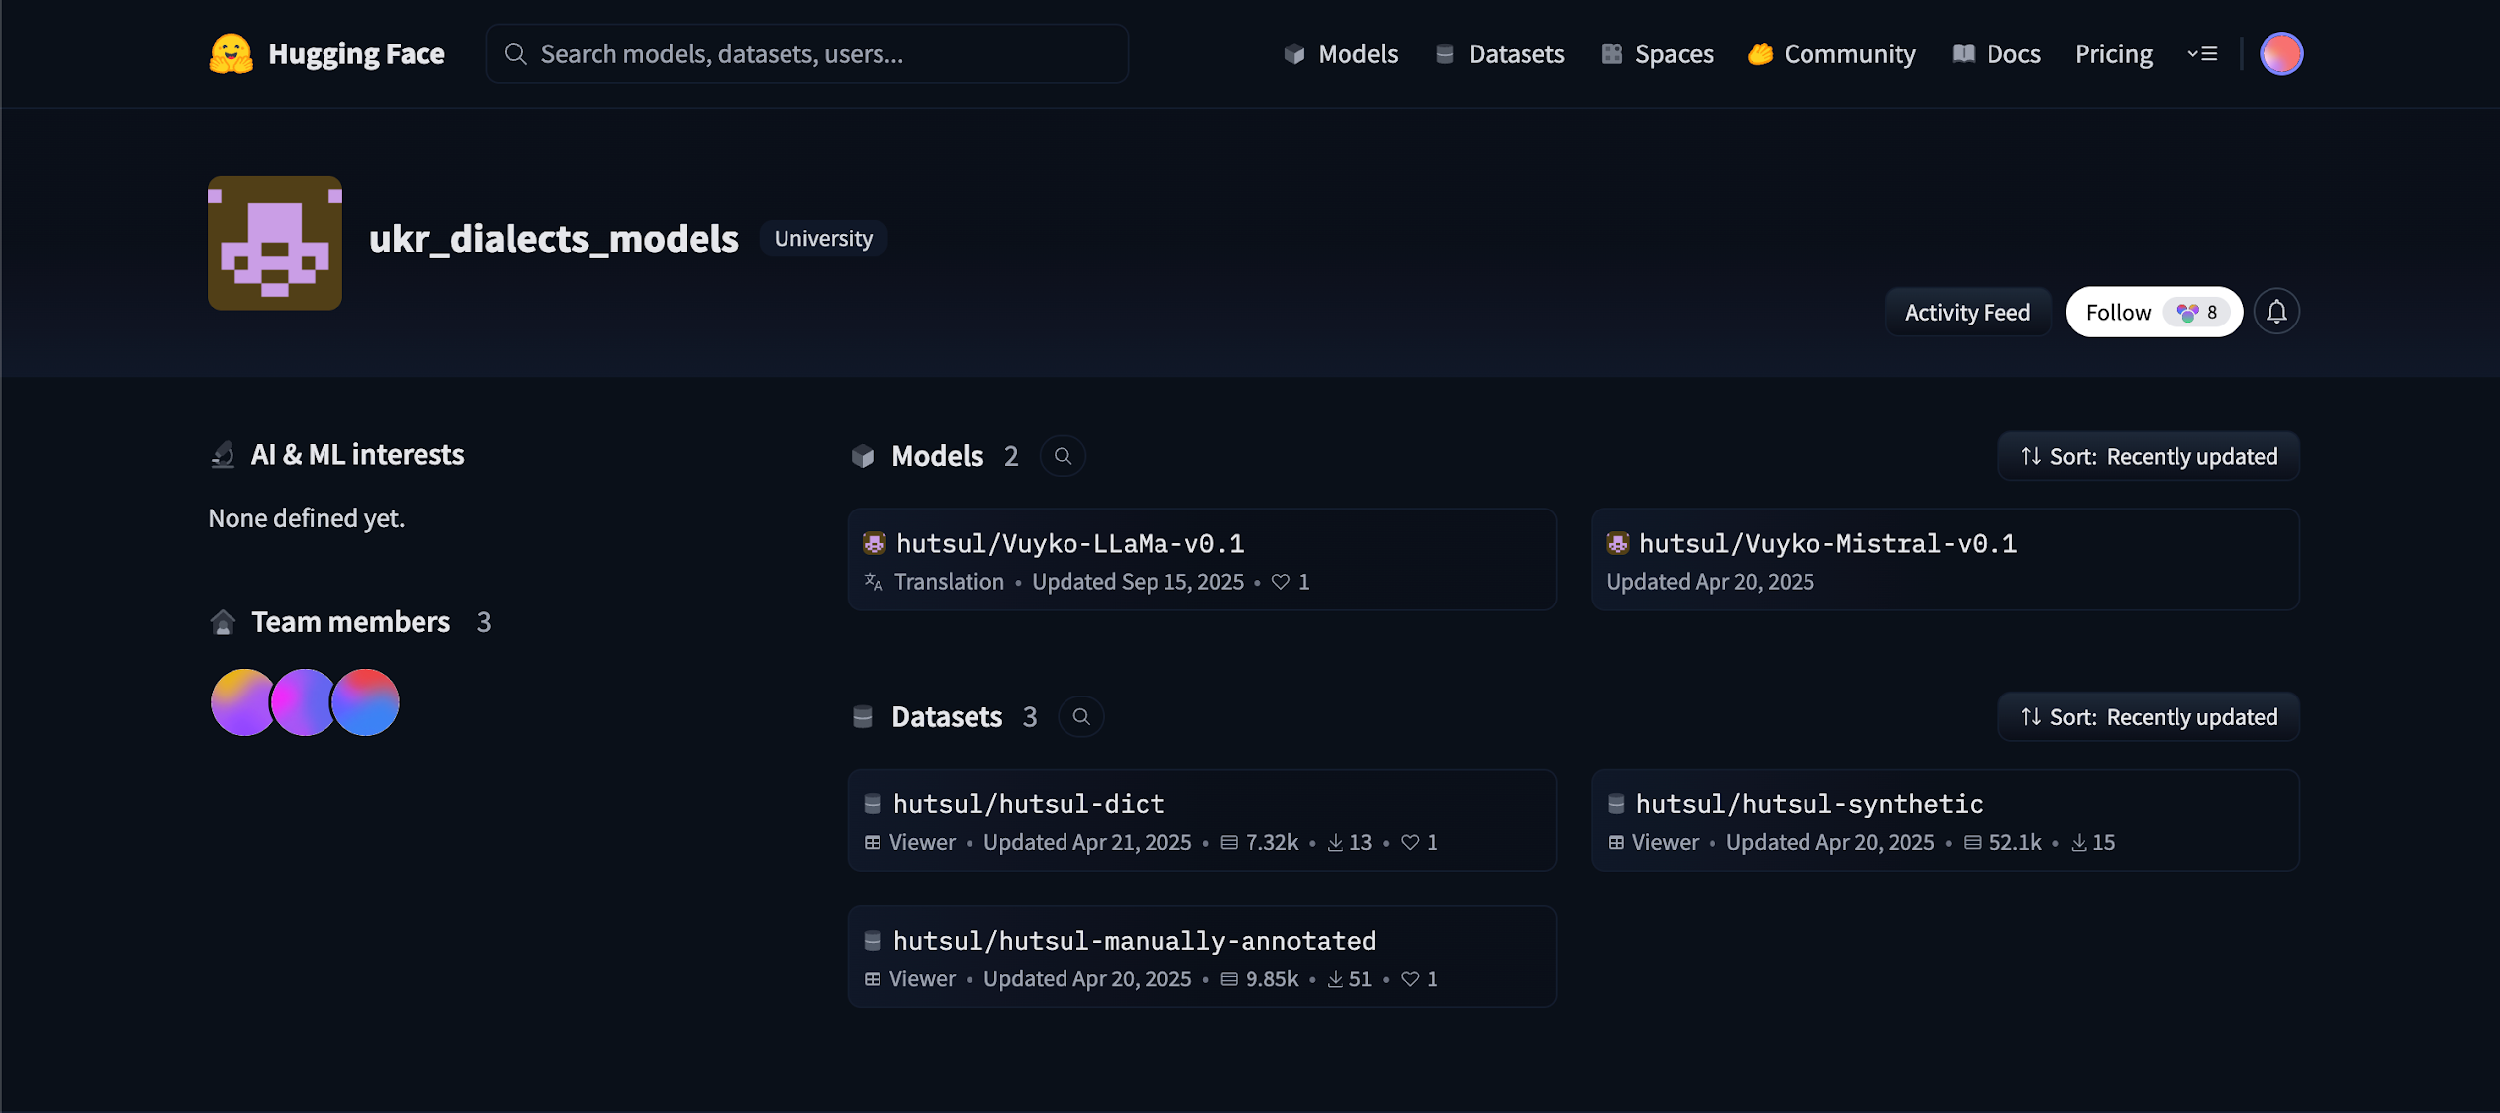
\includegraphics[width=0.9\textwidth]{images/1.1_hutsul_resources.png}
\caption{Гуцульські ресурси на платформі Hugging Face: датасети та допоміжні матеріали, що використовувались як вихідні джерела.}
\label{fig:hutsul_resources}
\end{figure}

Ручний корпус доповнено синтетично згенерованими парами: за допомогою моделі Mistral Small 24B з лінгвістичними правилами гуцульського діалекту отримано 19~841 пару. Таким чином, загальний обсяг гуцульської підвибірки в навчальному наборі склав 29~438 прикладів.

Діалектний словник виконував кілька функцій: слугував джерелом лексичних відповідників під час синтетичної генерації, обмежував простір допустимих діалектних замін і використовувався для валідації згенерованих пар - якщо у вхідному тексті були діалектні слова, перевірялась їх наявність у словнику. Словник містить 7~320 записів у форматі «діалектна форма - стандартна форма - словникова лема».

На рис.~\ref{fig:parallel_corpus} показано приклад вмісту вручну анотованого корпусу: кожен рядок містить вхідний діалектний текст і відповідний літературний еталон. У задачі нормалізації один діалектний вираз може мати кілька допустимих літературних варіантів, тому ручна розмітка фіксує один узгоджений еталон.

\begin{figure}[ht]
\centering
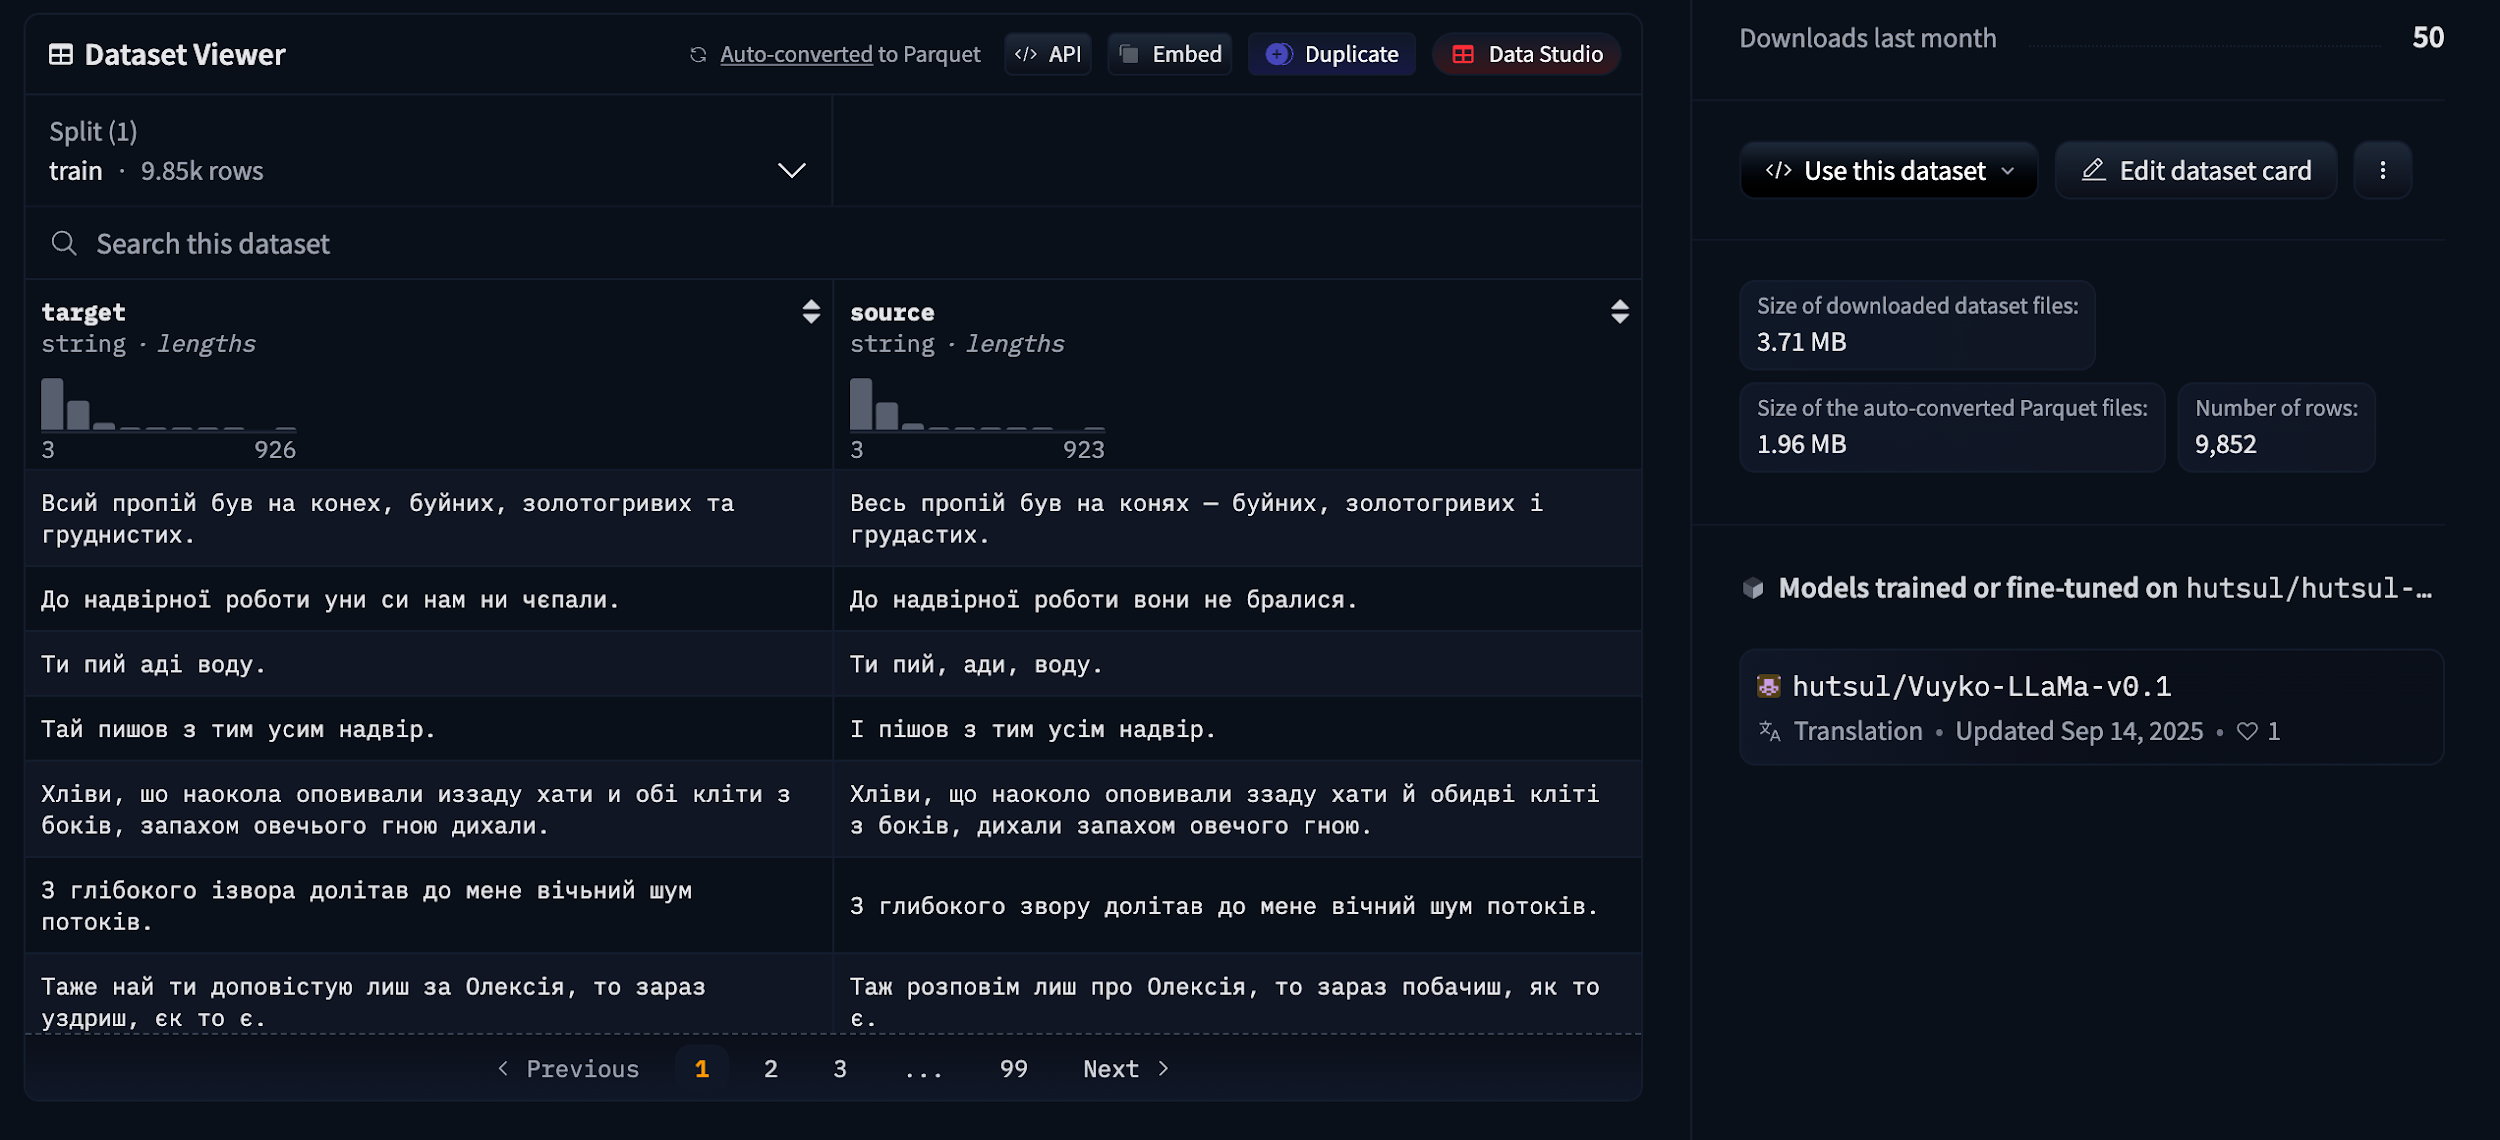
\includegraphics[width=0.9\textwidth]{images/1.2_parallel_corpus.png}
\caption{Вміст вручну анотованого паралельного корпусу для гуцульського діалекту: стовпці вхідного тексту та еталонного відповідника.}
\label{fig:parallel_corpus}
\end{figure}

\subsubsection{Корпус «Співавтор» як джерело літературної норми}

Для суржику еталонні речення літературної норми взято з корпусу «Співавтор» (рис.~\ref{fig:spivavtor}) - набору пар редагування і перефразування українською мовою, що охоплює виправлення граматичних помилок, перефразування і спрощення тексту~\citeref{ref:spivavtor}. У контексті цієї роботи «Співавтор» використовувався не як діалектний ресурс, а як пул стилістично природних літературних речень: з нього відбирались цільові речення, на основі яких генерувався суржиковий варіант.

\begin{figure}[ht]
\centering
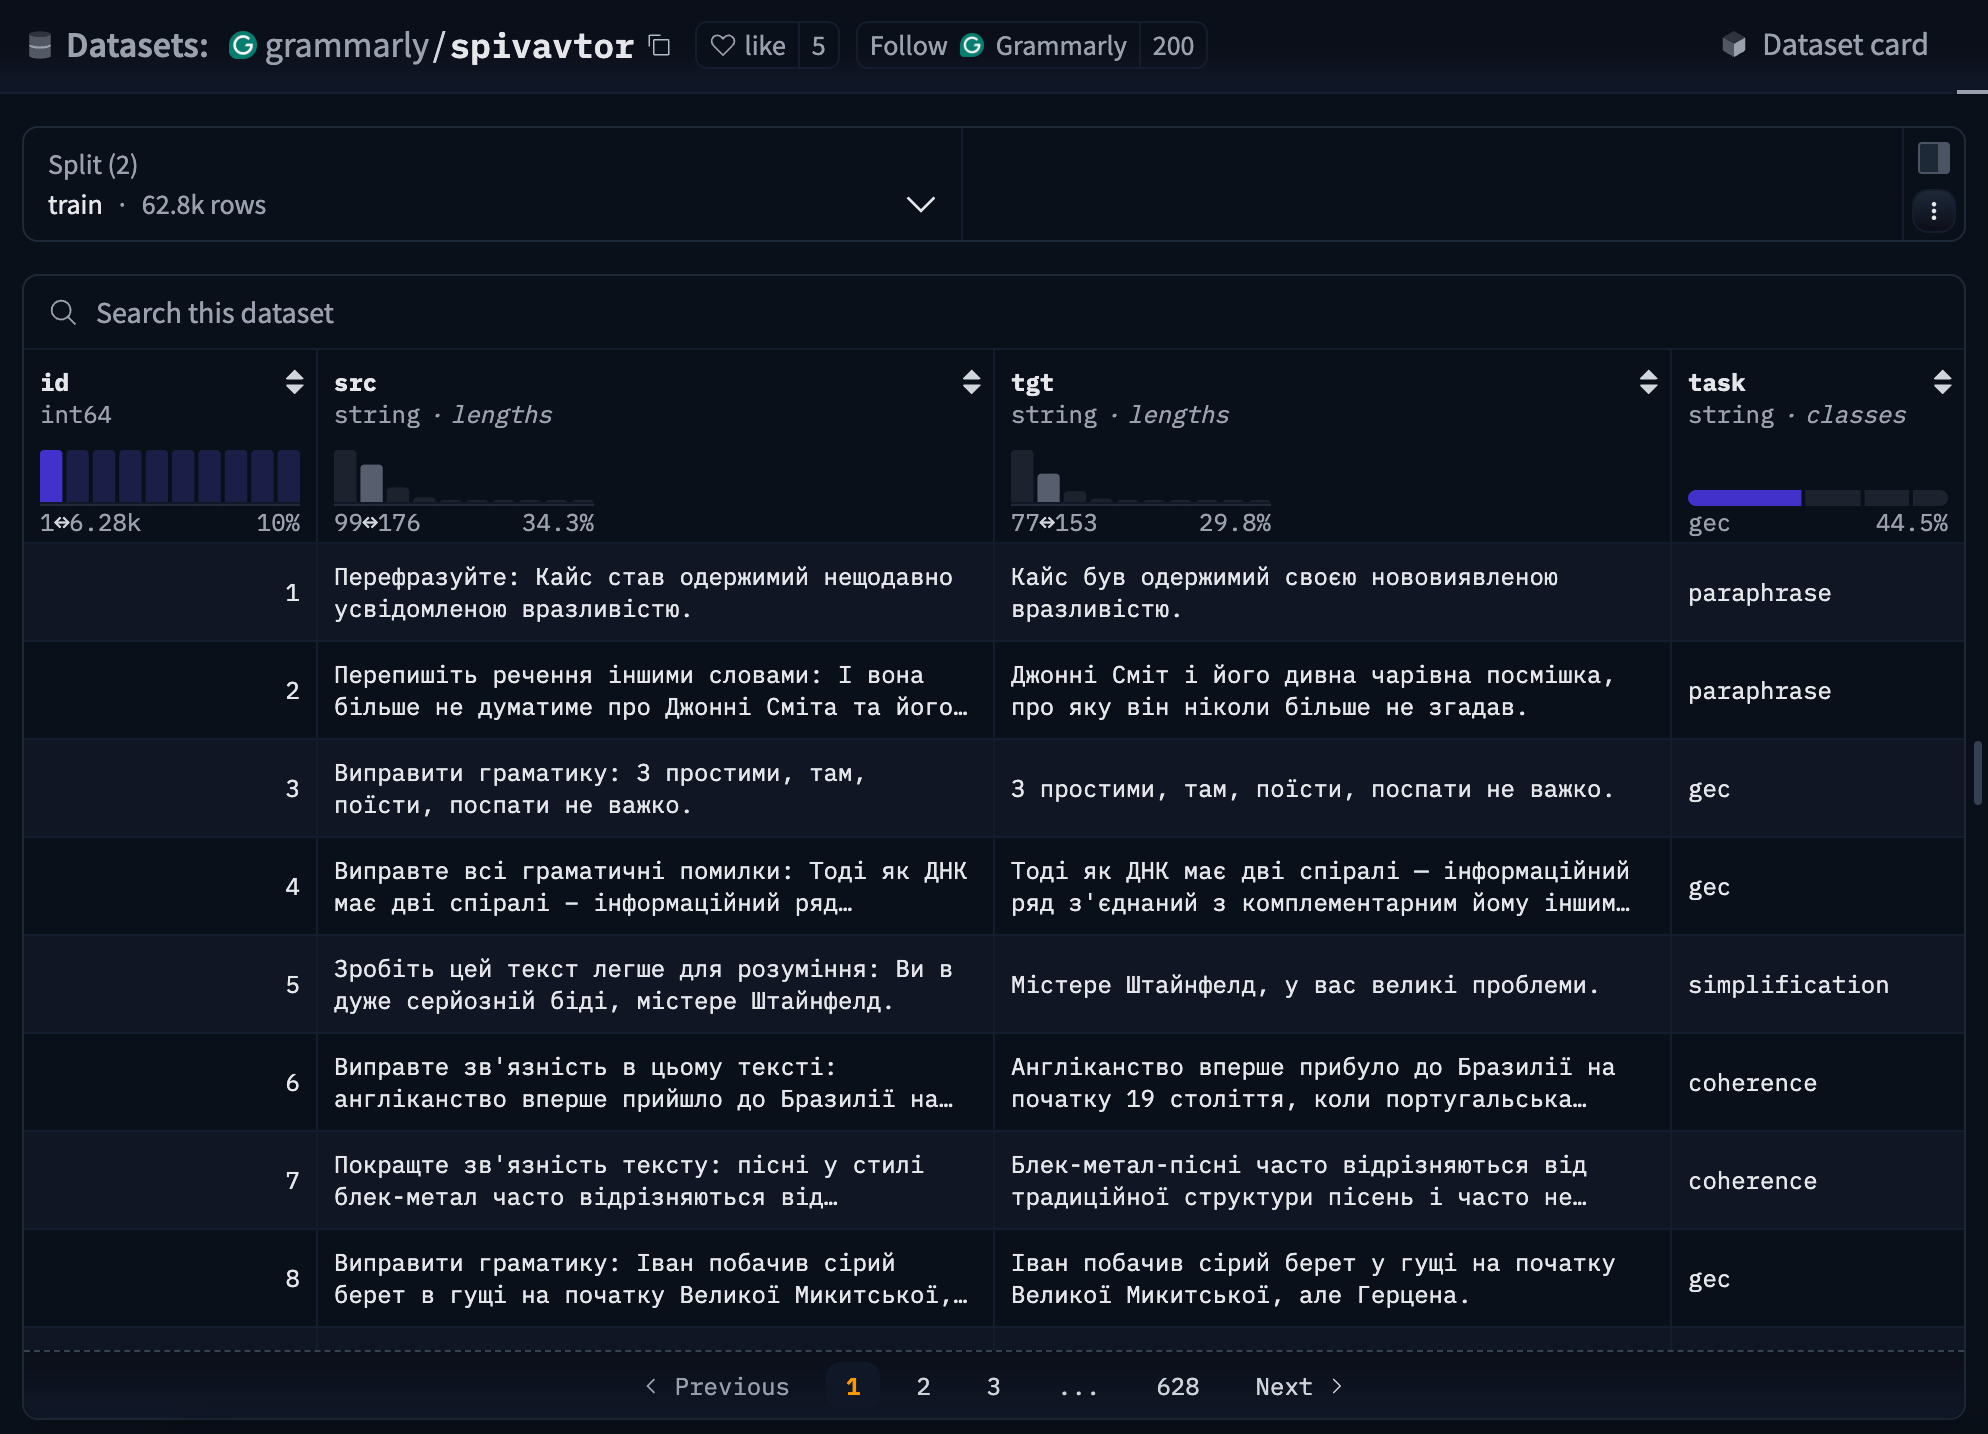
\includegraphics[width=0.9\textwidth]{images/1.3_spivavtor_dataset.png}
\caption{Приклад вмісту корпусу «Співавтор»: вхідний і відредагований текст із міткою типу завдання.}
\label{fig:spivavtor}
\end{figure}

Практична логіка така: обирається літературне речення $y$ зі «Співавтора», після чого генерується суржиковий варіант $x$. Таким чином пара $(x, y)$ гарантовано має якісний еталон. Перевага такого підходу полягає ще й у тому, що «Співавтор» містить широкий спектр природних речень із різних доменів - новини, побутові тексти, публіцистика, - що забезпечує доменну різноманітність навчальних прикладів для суржику.

\subsubsection{Словникова база мовних різновидів}

Для кожного з чотирьох мовних різновидів зібрано словники відповідників між діалектними і стандартними формами. Словники виконували подвійну роль у системі: слугували джерелом прикладів для шаблонів запитів до ВМM та засобом контролю якості згенерованих пар. Основні характеристики словників наведено в таблиці~\ref{tab:dicts}.

\begin{table}[ht]
\caption{Словники діалектних відповідників}
\label{tab:dicts}
\setlength{\tabcolsep}{4pt}
\begin{tabular}{|p{0.24\textwidth}|p{0.12\textwidth}|p{0.48\textwidth}|}
\hline
\textbf{Мовний різновид} & \textbf{Записів} & \textbf{Формат запису} \\
\hline
Гуцульський & 7~320 & Діалектна форма, стандартна форма, лема \\
\hline
Бойківський & 14~910 & Діалектна форма, стандартна форма, лема \\
\hline
Закарпатський & 7~469 & Діалектна форма, стандартна форма, лема \\
\hline
Суржик & 570 & Суржикова форма, стандартна форма \\
\hline
\end{tabular}
\end{table}

Бойківський словник є найбільшим (14~910 записів), що відображає значну лексичну відстань між бойківськими формами і стандартом. Словник суржику суттєво менший (570 записів), оскільки основні відхилення суржику є морфологічними і фонетичними (зміна закінчень, фонетичні кальки), а не лексичними замінами: для таких перетворень застосовується морфологічний аналізатор, а не словникова таблиця. Під час синтетичної генерації до кожного запиту включалось 3-5 прикладів із відповідного словника, що допомагало моделі дотримуватися лінгвістичного стилю конкретного діалекту.

\subsubsection{Синтетична генерація даних}

Для більшості мовних різновидів ручних паралельних даних критично мало, тому синтетичне розширення є необхідним. У роботі застосовано підхід «норма $\to$ нестандарт»: за вхідний еталон $y$ береться літературне речення, а нестандартний варіант $x$ генерується. Це зручно, бо якість еталону гарантована від початку.

\textit{Правилова генерація суржику.} Реалізовано двофазову заміну. На першій фазі здійснюється фразова заміна: за допомогою регулярних виразів виявляються найдовші збіги із словником багатослівних суржикових конструкцій і замінюються їхніми еквівалентами (наприклад, «тому що» $\to$ «потому шо»). Ця фаза обробляє контекстні сполучення до розбиття тексту на окремі слова. На другій фазі виконується морфологічна заміна на рівні слів: кожне слово лематизується через бібліотеку морфологічного аналізу pymorphy2, і якщо словникова лема входить до списку замін суржику, відповідне слово замінюється з урахуванням граматичних категорій - відмінку, числа і роду. Такий підхід забезпечує не просто лексичну, а морфологічно узгоджену заміну і дав 20~911 прикладів.

\textit{Генерація за допомогою ВМM.} Застосована для всіх чотирьох мовних різновидів. Для кожного діалекту підготовлено окремий системний запит, що містить лінгвістичний опис типових рис, 3-5 демонстраційних пар зі словника та інструкцію щодо кількості і стилю замін. Велика мовна модель Mistral Small 24B (4-бітна квантизація для локальної інференції) обробляла пакети по 5-10 речень і повертала діалектні варіанти. Приклад шаблону запиту зображено на рис.~\ref{fig:prompt_template}.

\begin{figure}[ht]
\centering
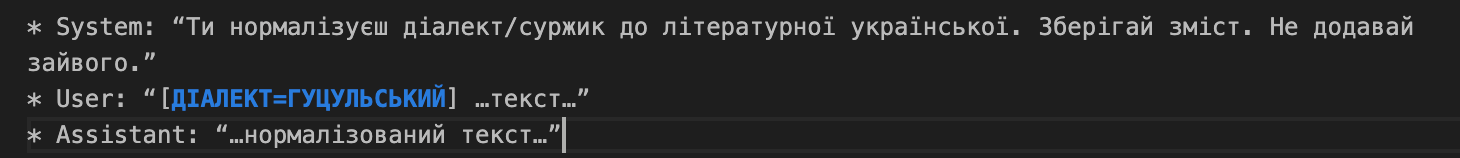
\includegraphics[width=0.9\textwidth]{images/2.2_prompt_template.png}
\caption{Приклад шаблону запиту для синтетичної генерації діалектних пар: інструкція, правила діалекту і демонстраційні приклади.}
\label{fig:prompt_template}
\end{figure}

Контроль якості синтетичних пар проводився після кожного пакету: видалялись дублікати (однакові вхідні або еталонні тексти), відкидались надто короткі (менше трьох слів) та надто довгі пари, перевірялась наявність діалектних слів зі словника у вхідному тексті, вибірково проводився ручний перегляд для оцінки типових артефактів генерації - змішування мов, незавершених речень, залишків форматування у відповіді.

\subsubsection{Формування та структура фінального корпусу}

Після генерації всіх складових дані об'єднано в єдиний корпус і розділено на три вибірки. Загальна структура наведена в таблиці~\ref{tab:corpus}.

\begin{table}[ht]
\caption{Склад паралельного корпусу по мовних різновидах}
\label{tab:corpus}
\setlength{\tabcolsep}{4pt}
\begin{tabular}{|p{0.21\textwidth}|p{0.13\textwidth}|p{0.14\textwidth}|p{0.18\textwidth}|p{0.18\textwidth}|}
\hline
\textbf{Різновид} & \textbf{Ручні} & \textbf{LLM} & \textbf{Правилові} & \textbf{Разом} \\
\hline
Гуцульський & 9~853 & 19~841 & - & 29~694 \\
\hline
Бойківський & - & 29~754 & - & 29~754 \\
\hline
Закарпатський & - & 29~605 & - & 29~605 \\
\hline
Суржик & - & 29~612 & 20~911 & 50~523 \\
\hline
\textbf{Разом} & \textbf{9~853} & \textbf{108~812} & \textbf{20~911} & \textbf{139~576} \\
\hline
\end{tabular}
\end{table}

Після формування загального об'єднаного набору 90\% прикладів виділено у навчальну вибірку (125~615 прикладів), 10\% - у валідаційну (13~756 прикладів). Тестова вибірка з 200 прикладів (по 50 на кожен мовний різновид) сформована виключно з вручну анотованих пар, що забезпечує об'єктивність оцінювання і виключає вплив якості синтетичного генератора на тестові метрики.

Ключовий принцип організації: тестова і валідаційна вибірки формуються лише з ручних пар, синтетика використовується виключно в навчальній вибірці. Це дозволяє уникнути переоцінки якості на штучних прикладах і отримувати метрики, близькі до реального застосування. Структуру директорій репозиторію і розміщення файлів корпусу показано на рис.~\ref{fig:project_structure}.

\begin{figure}[ht]
\centering
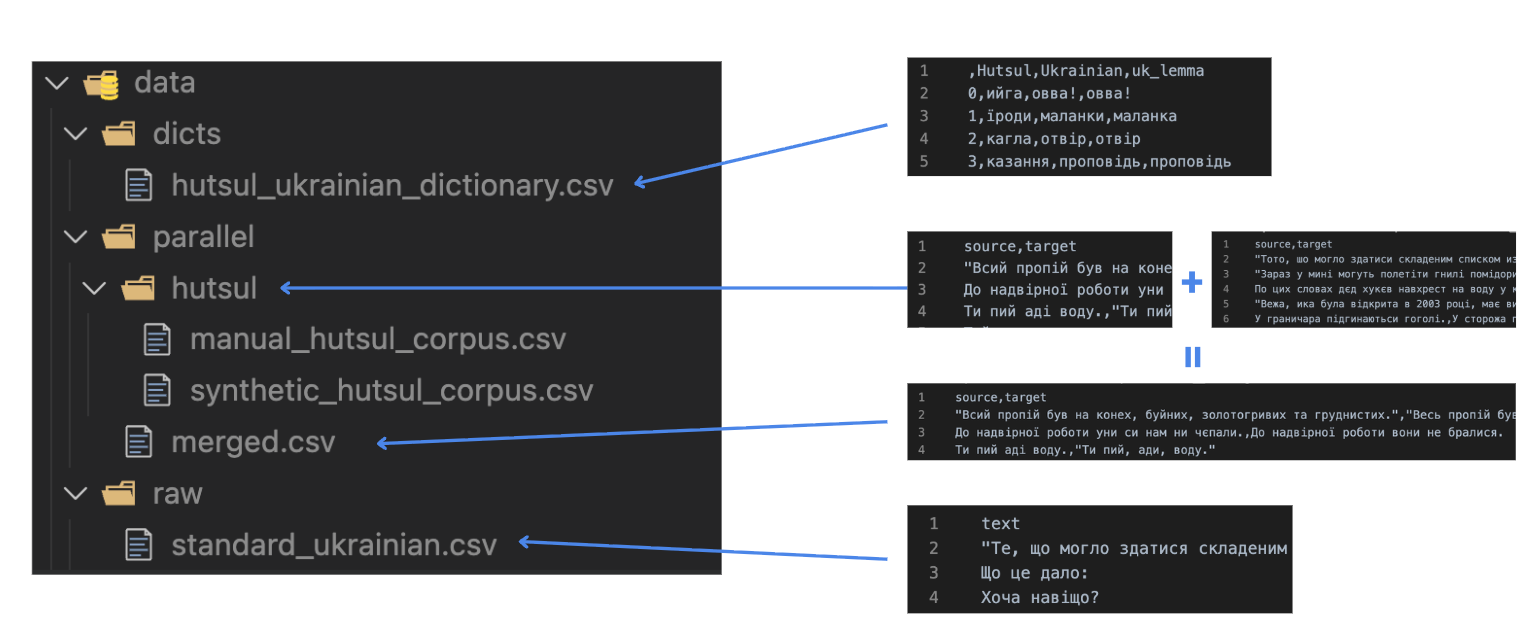
\includegraphics[width=0.8\textwidth]{images/1.4_project_structure.png}
\caption{Структура директорій проєкту: словники, ручні корпуси, синтетичні дані та фінальні вибірки для навчання, валідації і тестування.}
\label{fig:project_structure}
\end{figure}

\subsection{Висновки до розділу~1}

У розділі проаналізовано предметну галузь, розглянуто суміжні дослідження та сформовано корпус для навчання системи.

Нормалізація діалектів і суржику є задачею на межі між НМП і виправленням граматичних помилок: тут присутні як систематичні лексичні заміни, так і фонетичні та морфологічні трансформації регулярного характеру. Аналіз літератури показав: для малоресурсних сценаріїв синтетичне розширення даних і донавчання ВМM є ефективними підходами, а для українських діалектів і суржику до цього часу не існувало спеціалізованих паралельних корпусів і моделей нормалізації.

Чотири досліджуваних різновиди суттєво відрізняються за природою відхилень: гуцульський і бойківський є регіональними діалектами з архаїчними фонологічними рисами, закарпатський демонструє контактний вплив суміжних мов, суржик є соціолінгвістичним явищем змішаного мовлення.

Зібрано паралельний корпус із 139~576 прикладів загалом, з яких 125~615 увійшли до навчальної вибірки. Для гуцульського діалекту використано ручний корпус (9~853 пари) і словник (7~320 записів). Для бойківського і закарпатського словники містять 14~910 і 7~469 записів відповідно. Суржиковий корпус отримано поєднанням правилового підходу (20~911 прикладів) і генерації за допомогою ВМM (29~612). Тестові вибірки сформовано виключно з ручних пар, що забезпечує надійне оцінювання якості у наступних розділах.

\clearpage

% -------- розділ 2 --------
\section{ІНФОРМАЦІЙНЕ ТА МАТЕМАТИЧНЕ ЗАБЕЗПЕЧЕННЯ}

Розділ містить формалізацію задачі нормалізації, опис двох підходів (seq2seq та decoder-only LLM), обґрунтування вибору архітектур, а також математичні основи навчання, декодування та оцінювання. Узагальнену схему системи показано на рис.~\ref{fig:system_scheme}.

\begin{figure}[h]
\centering
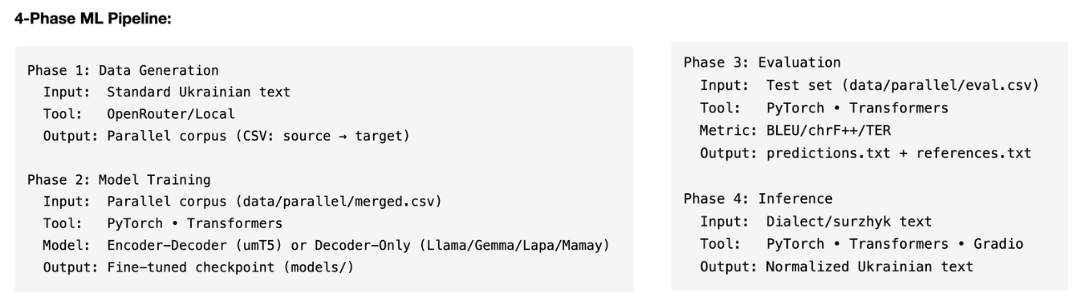
\includegraphics[width=0.9\textwidth]{images/2.1_system_scheme.png}
\caption{Узагальнена схема системи: (а) базова модель ``гуцульський $\to$ літературна'', (б) мультидіалектний і суржиковий етап на MamayLM, (в) демо-інтерфейс.}
\label{fig:system_scheme}
\end{figure}

\subsection{Аналіз методів і підходів до нормалізації діалектів та суржику}

\subsubsection{Нормалізація як задача перетворення тексту}

Нормалізацію діалектних форм та суржику можна розглядати як кероване перетворення тексту, де необхідно зберегти зміст, але змінити форму (лексичну, морфологічну, орфографічну, інколи синтаксичну) відповідно до літературної норми. На відміну від «виправлення граматики» у вузькому сенсі, тут часто присутні лексичні заміни (діалектизми), варіативна орфографія, фонетично мотивовані написання, а також перемикання мов (для суржику).

Формально будемо мати вхідний рядок $x$ (діалект/суржик) та бажаний вихідний рядок $y$ (літературна українська). Мета - побудувати модель $f_\theta$, що апроксимує відображення:
\[f_\theta: x \mapsto y\]

З погляду статистичного моделювання це еквівалентно оцінюванню умовного розподілу $p_\theta(y|x)$.

Практичні особливості задачі:
\begin{itemize}
  \item часткова тотожність: значна частина токенів у $x$ може збігатися з $y$;
  \item асиметрія трансформацій: ``виправляти занадто багато'' небезпечно (ризик спотворити зміст), але ``виправляти занадто мало'' - не виконати нормалізацію;
  \item багатоваріантність норми: одна діалектна форма може мати декілька літературних парафразів;
  \item низькоресурсність: для більшості діалектів немає великих вручну розмічених паралельних корпусів.
\end{itemize}

\subsubsection{Правилові підходи та їх обмеження}

Правилова нормалізація опирається на словники відповідників, регулярні правила перетворень і евристики. Її перевага - контрольованість і пояснюваність: якщо відомі правила заміни, можна гарантувати певну поведінку. Однак для українських діалектів і суржику правиловий підхід зазвичай має такі проблеми:
\begin{itemize}
  \item складно охопити всю лексичну варіативність;
  \item важко правильно моделювати контекстні значення (омонімія/полісемія);
  \item правила погано працюють із довгими залежностями і перебудовами;
  \item якість деградує при зміні домену (побутові чати, оголошення, студентські конспекти тощо).
\end{itemize}

Тому rule-based ресурси (словники/правила) у цій роботі розглядаються як допоміжні: (а) для побудови синтетичних даних; (б) для підказок (retrieval) під час генерації синтетики; (в) як інструмент аналізу помилок.

\subsubsection{Нейромережеві підходи: seq2seq і decoder-only LLM}

У роботі послідовно застосовано дві парадигми.

\textbf{1. Seq2seq (encoder-decoder) для бейзлайну на одному діалекті (гуцульському).}

Переваги:
\begin{itemize}
  \item стабільне навчання на паралельних даних;
  \item природна постановка як ``переклад'' $x \to y$;
  \item добре підходить для невеликих/середніх моделей і обмежених ресурсів.
\end{itemize}

\textbf{2. Decoder-only LLM (instruction-tuned) для розширення на багато діалектів і суржик.}

Переваги:
\begin{itemize}
  \item універсальність: одна модель може виконувати різні підзадачі (нормалізація різних діалектів, суржик, пояснення правок);
  \item простіший формат даних через інструкції (prompt $\to$ response);
  \item потенційно краща генеративна ``плинність'' та стилістична якість.
\end{itemize}

Ключовою базовою моделлю для масштабування обрано Lapa LLM, оскільки це відкрита українсько-орієнтована LLM, побудована на базі Gemma-3-12B та оптимізована під українську за рахунок адаптації токенізатора і прозорого пайплайна тренування~\citeref{ref:lapallm}.

\subsection{Постановка задачі та інформаційна модель даних}

\subsubsection{Формальна постановка}

Нехай $\Sigma$ - алфавіт символів (або множина байтів/токенів), тоді вхідний текст:
\[x = (x_1, x_2, \ldots, x_{|x|}), \quad x_i \in \Sigma\]

вихідний текст:
\[y = (y_1, y_2, \ldots, y_{|y|}), \quad y_j \in \Sigma\]

Задача - знайти параметри $\theta$, що максимізують правдоподібність тренувальних пар $\{(x^{(k)}, y^{(k)})\}_{k=1}^N$:
\[\theta^* = \arg\max_\theta \sum_{k=1}^N \log p_\theta(y^{(k)}|x^{(k)})\]

У практичній реалізації використовується мінімізація негативного лог-правдоподібності (крос-ентропії):
\[L(\theta) = -\sum_{k=1}^N \log p_\theta(y^{(k)}|x^{(k)})\]

\subsubsection{Подання даних для seq2seq}

Для encoder-decoder моделі дані зберігаються у вигляді пар:
\begin{itemize}
  \item source: діалект/суржик;
  \item target: літературна українська.
\end{itemize}

Після токенізації отримуємо послідовності індексів $x = (x_1, \ldots, x_T)$, $y = (y_1, \ldots, y_{T'})$. Модель навчається прогнозувати $y_t$ з урахуванням усіх $x$ та попередніх $y_{<t}$:
\[p_\theta(y|x) = \prod_{t=1}^{T'} p_\theta(y_t|x, y_{<t})\]

\subsubsection{Подання даних для instruction-tuned LLM (chat format)}

Для decoder-only LLM зручно представляти задачу як інструкцію, де модель отримує:
\begin{itemize}
  \item роль ``system'' із правилами нормалізації;
  \item роль ``user'' із текстом (і, за потреби, міткою діалекту/режиму);
  \item роль ``assistant'' із відповіддю-нормою (рис.~\ref{fig:chat_format}).
\end{itemize}

\begin{figure}[h]
\centering
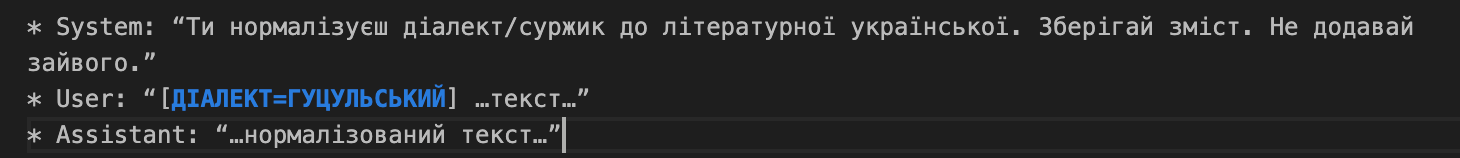
\includegraphics[width=0.8\textwidth]{images/2.2_prompt_template.png}
\caption{Приклад шаблону інструкції для декодерної ВМM: system/user/assistant та місце для маркера діалекту.}
\label{fig:chat_format}
\end{figure}

\subsection{Математичні основи використаних моделей}

\subsubsection{Архітектура Transformer: увага та обчислення}

Основою і для seq2seq, і для decoder-only підходів є Transformer, який використовує механізм самоуваги. Нехай на вході є матриця представлень токенів $H \in \mathbb{R}^{T \times d}$. Для одного attention-блоку обчислюються:
\[Q = HW_Q, \quad K = HW_K, \quad V = HW_V\]

де $W_Q, W_K, W_V \in \mathbb{R}^{d \times d_k}$.

Далі:
\[\text{Attention}(Q, K, V) = \text{softmax}\left(\frac{QK^T}{\sqrt{d_k}}\right)V\]

Multi-head attention використовує кілька голів і конкатенацію результатів:
\[\text{MHA}(H) = \text{Concat}(\text{head}_1, \ldots, \text{head}_h)W_O\]

\subsubsection{Seq2seq encoder-decoder: умовна генерація}

Encoder перетворює вхід $x$ у контекстні представлення $E$. Decoder генерує $y$, використовуючи:
\begin{itemize}
  \item self-attention по вже згенерованих токенах,
  \item cross-attention до $E$.
\end{itemize}

\subsubsection{Decoder-only LLM: автогресивна модель}

Decoder-only LLM моделює послідовність токенів $z$ (де $z$ включає system+user+assistant у вигляді одного ``ланцюжка''):
\[p_\theta(z) = \prod_{t=1}^{|z|} p_\theta(z_t|z_{<t})\]

На практиці нас цікавить якість саме на токенах відповіді assistant, тому під час навчання можна маскувати loss так, щоб оптимізувати лише частину ``assistant''.

\subsection{Вибір моделі та обґрунтування: від бейзлайну до Lapa LLM}

\subsubsection{Бейзлайн для гуцульського діалекту як необхідний етап}

Першим етапом реалізовано бейзлайн для гуцульського діалекту - з трьох причин:
\begin{enumerate}
  \item дозволяє перевірити, що паралельні дані, токенізація та навчання працюють коректно;
  \item дає контрольований ``полігон'' для аналізу помилок;
  \item створює поріг якості, від якого можна вимірювати виграш при переході до LLM (рис.~\ref{fig:baseline_training}).
\end{enumerate}

\begin{figure}[h]
\centering
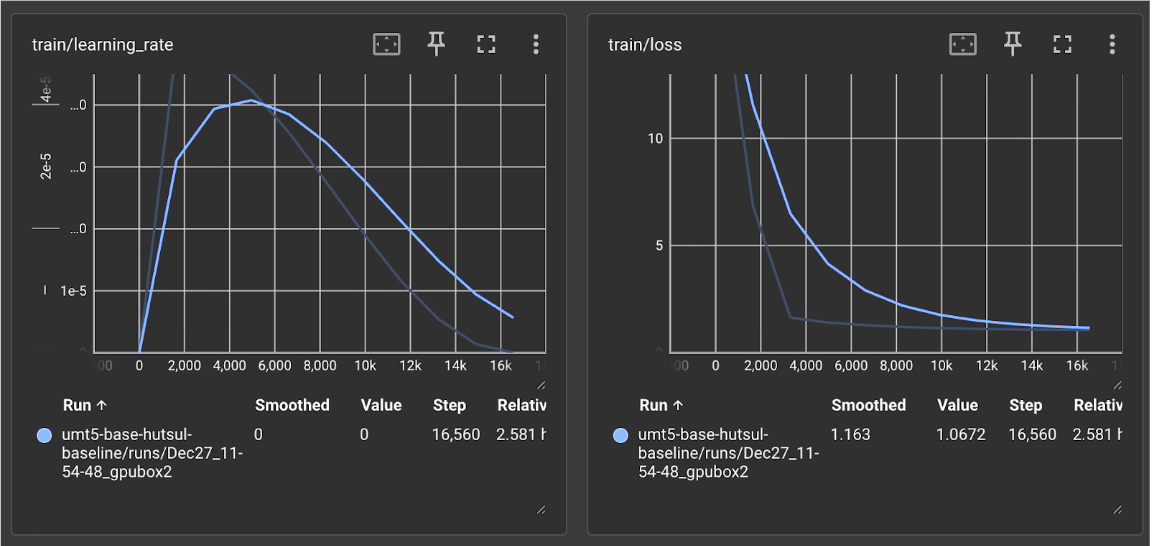
\includegraphics[width=0.9\textwidth]{images/2.3_baseline_training.png}
\caption{Графік навчання бейзлайну (learning rate та loss).}
\label{fig:baseline_training}
\end{figure}

Результати оцінювання якості бейзлайну на валідаційній вибірці показано на рис.~\ref{fig:baseline_eval}. Метрика BLEU стабілізується на рівні ~51, що свідчить про адекватність моделі для задачі нормалізації.

\begin{figure}[h]
\centering
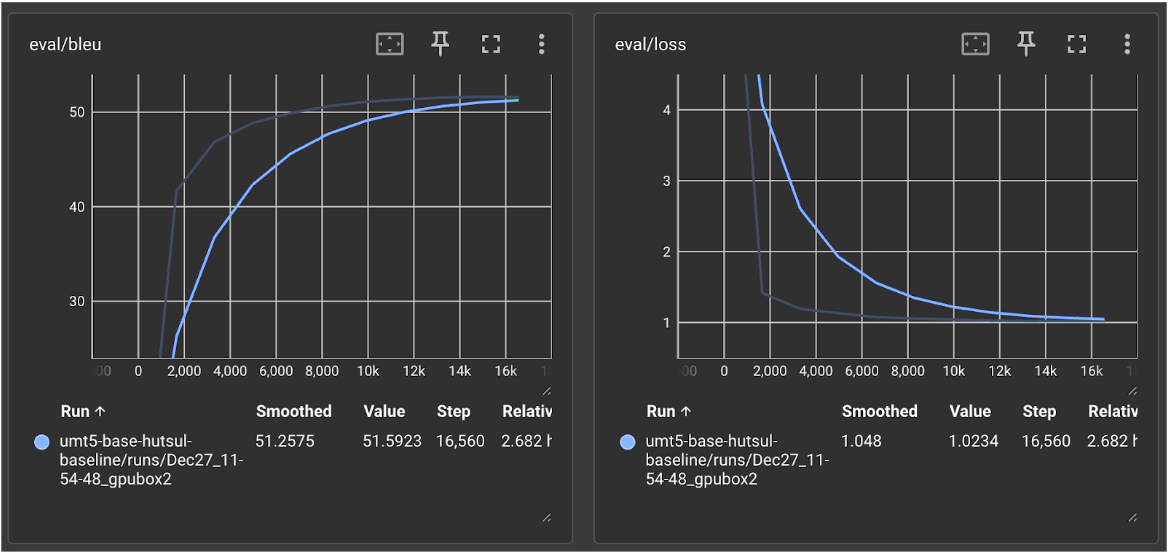
\includegraphics[width=0.9\textwidth]{images/2.4_baseline_eval.png}
\caption{Результати оцінювання бейзлайну: метрика BLEU (ліворуч) та validation loss (праворуч) під час навчання.}
\label{fig:baseline_eval}
\end{figure}

\subsubsection{Масштабування на мультидіалектність і суржик}

Перехід від одного діалекту до множини діалектів та суржику ускладнює задачу:
\begin{itemize}
  \item зростає різноманітність фонетичних і лексичних явищ;
  \item з'являється потреба у ``перемикачі'' режимів (який діалект нормалізуємо);
  \item необхідна краща генеративна здатність для природного стилю.
\end{itemize}

Decoder-only LLM з інструкційним форматом природно підтримує цю постановку: можна додавати в prompt маркер діалекту або навіть просити модель самостійно визначити різновид і нормалізувати.

\subsubsection{Lapa LLM: ключові властивості}

Для мультидіалектного етапу використано Lapa LLM~\citeref{ref:lapallm} (рис.~\ref{fig:lapa_llm}) - відкриту українсько-орієнтовану модель, що базується на Gemma-3-12B.

Властивості, які прямо впливають на якість і ефективність нормалізації:
\begin{enumerate}
  \item \textbf{Український токенізатор} - замінено приблизно 80 тис. токенів із 250 тис. на українські, що дає скорочення кількості потрібних токенів приблизно у 1.5 раза.
  \item \textbf{Instruction-tuned версія} - спрощує інтеграцію в прикладний сервіс.
  \item \textbf{Довгий контекст} - підтримка до 128K токенів відкриває шлях до RAG-підходів.
  \item \textbf{Відкритість та відтворюваність} - публікується код і набори даних.
\end{enumerate}

\begin{figure}[h]
\centering
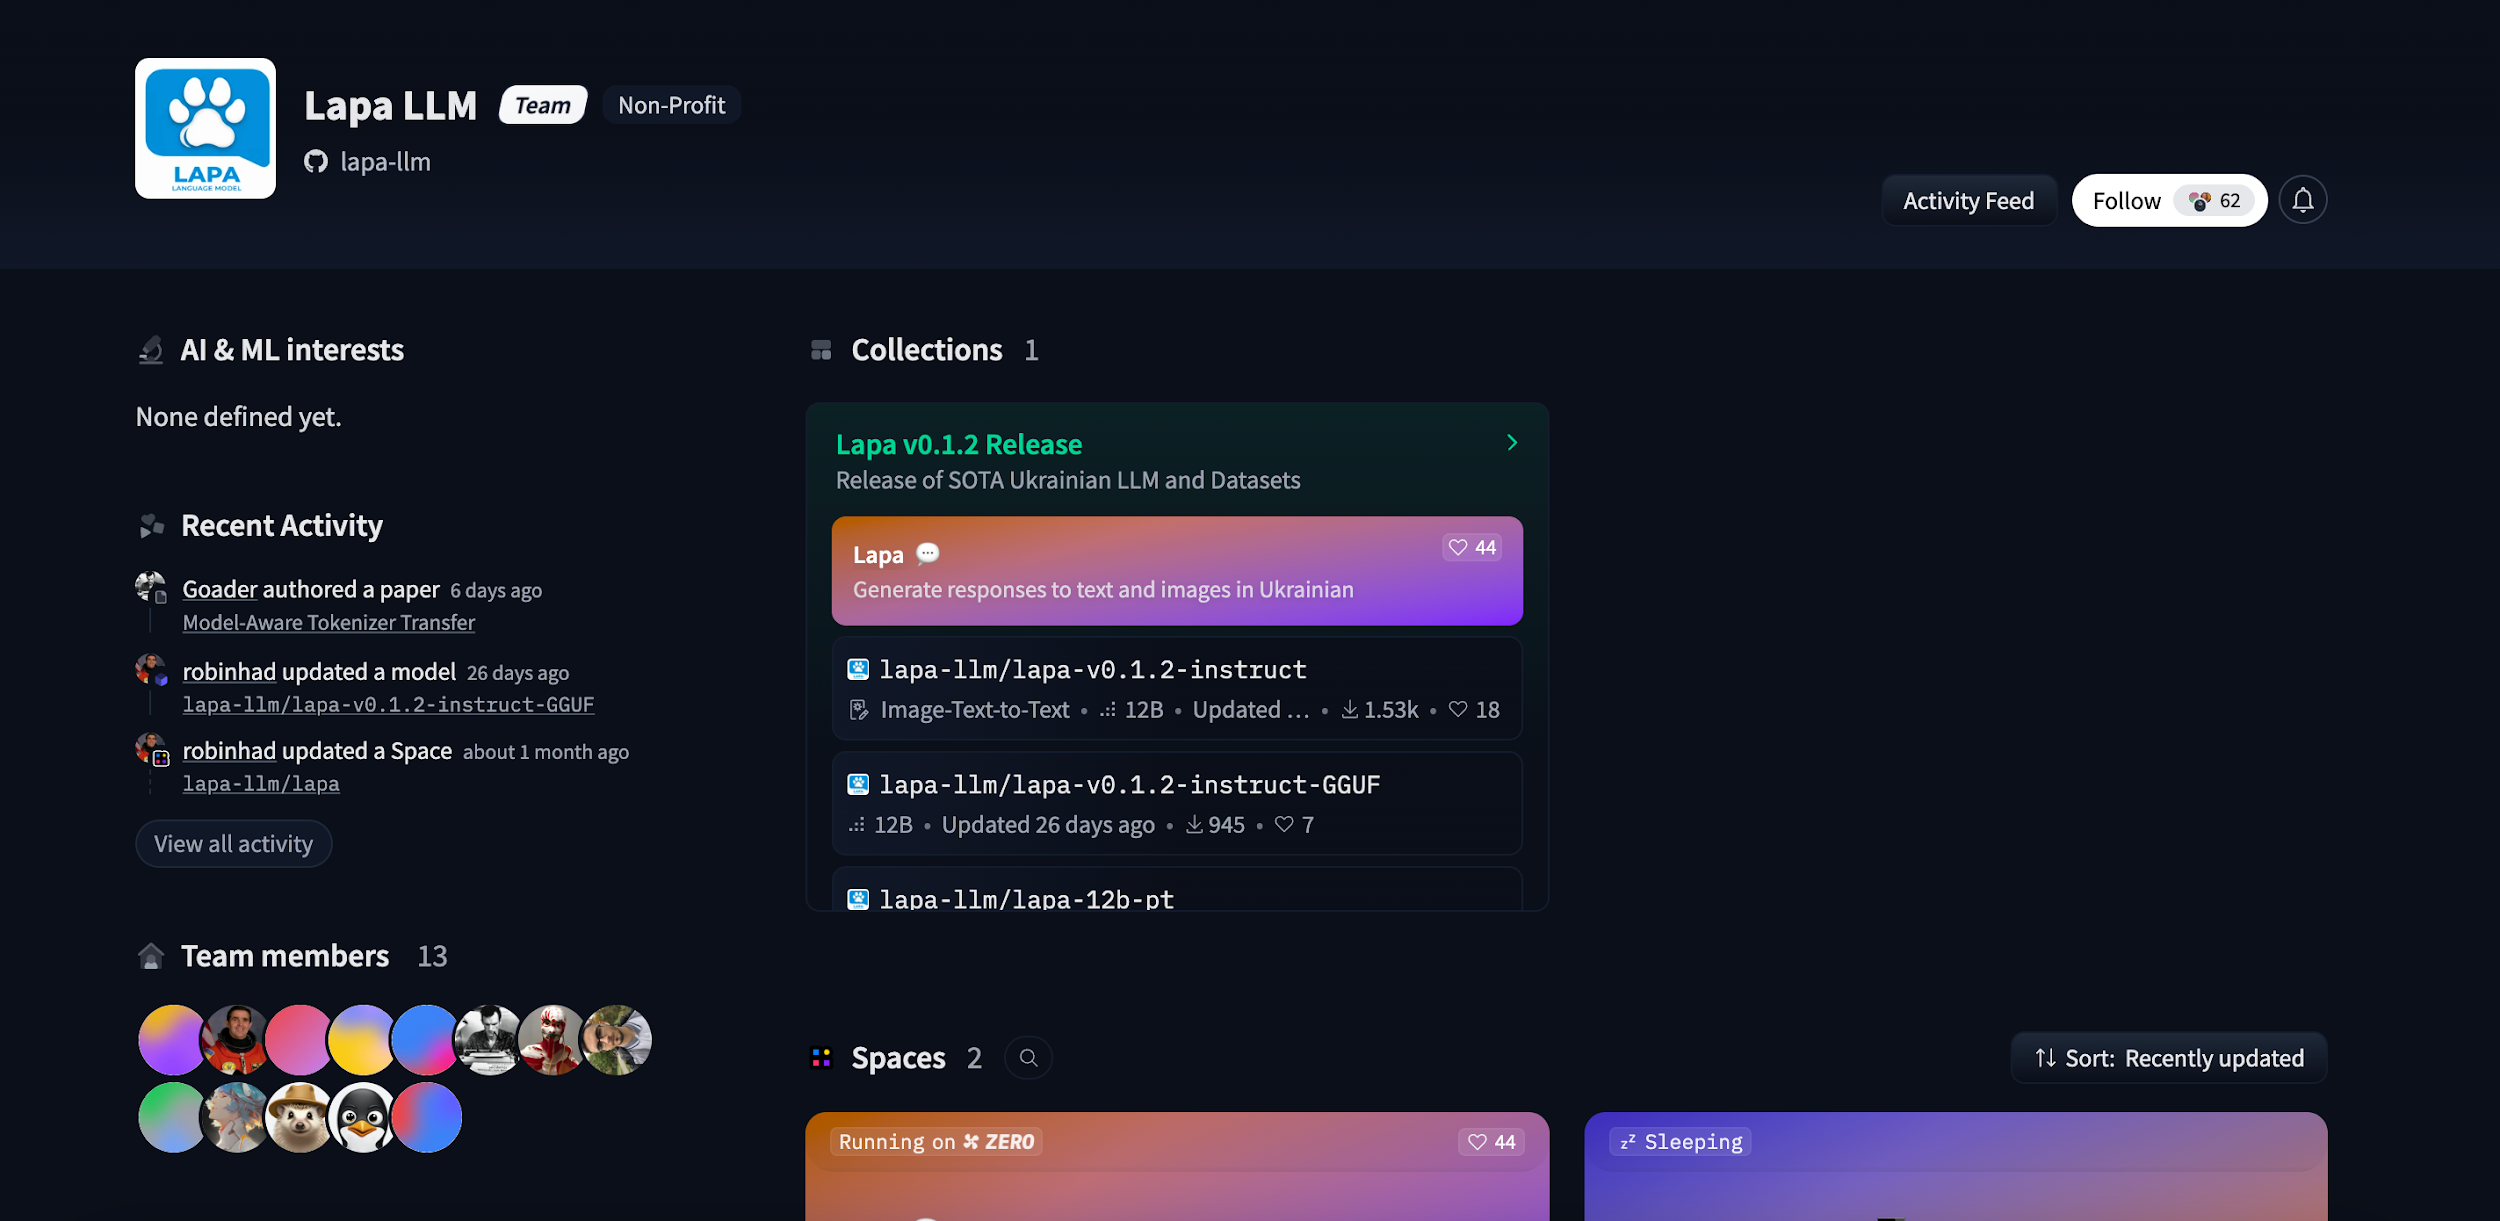
\includegraphics[width=0.8\textwidth]{images/2.5_lapa_llm.png}
\caption{Сторінка моделі Lapa LLM на Hugging Face.}
\label{fig:lapa_llm}
\end{figure}

\subsubsection{Параметро-ефективне донавчання LLM: LoRA/QLoRA}

Повне донавчання 12B-моделі є дорогим, тому практично застосовується PEFT (parameter-efficient fine-tuning), найчастіше LoRA (рис.~\ref{fig:lora}).

Нехай у Transformer є матриця ваг $W \in \mathbb{R}^{d \times k}$. LoRA додає низькорангову поправку:
\[W' = W + \Delta W, \quad \Delta W = BA\]
де $B \in \mathbb{R}^{d \times r}$, $A \in \mathbb{R}^{r \times k}$, а $r \ll \min(d, k)$.

Тоді кількість тренованих параметрів зменшується з $dk$ до $r(d+k)$.

\begin{figure}[h]
\centering
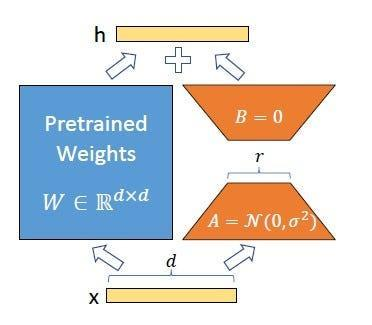
\includegraphics[width=0.5\textwidth]{images/2.6_lora.jpg}
\caption{Ілюстрація ідеї LoRA: замість повного оновлення ваг - низькорангова поправка в attention/FFN шарах.}
\label{fig:lora}
\end{figure}

\subsection{Метрики якості та цільові функції навчання}

\subsubsection{Крос-ентропія та маскування втрат}

Стандартна функція втрат для генеративних моделей:
\[L = -\sum_{t=1}^{T'} \log p_\theta(y_t|x, y_{<t})\]

Для instruction-tuned LLM доцільно оптимізувати лише токени відповіді assistant. Нехай $m_t \in \{0, 1\}$ - маска (1 лише на позиціях відповіді), тоді:
\[L_{masked} = -\sum_{t=1}^{T} m_t \log p_\theta(z_t|z_{<t})\]

\subsubsection{Декодування: greedy та beam search}

Під час інференсу потрібно знайти:
\[\hat{y} = \arg\max_y \log p_\theta(y|x)\]

Greedy-декодування:
\[\hat{y}_t = \arg\max_{y_t} p_\theta(y_t|x, \hat{y}_{<t})\]

Beam search підтримує $B$ найкращих часткових гіпотез. Часто застосовують штраф за довжину (length penalty).

\subsubsection{BLEU та chrF++ для нормалізації}

Оскільки задача близька до перекладу, застосовні метрики MT. BLEU базується на модифікованій n-грамній точності та штрафі за короткість:
\[\text{BLEU} = BP \cdot \exp\left(\sum_{n=1}^{N} w_n \log p_n\right)\]

де $p_n$ - модифікована точність n-грам, $w_n$ - ваги, а $BP$ (brevity penalty) штрафує за короткі гіпотези.

Для мов із багатою морфологією символьні метрики часто корисніші. chrF/chrF++ вимірює F-міру на символьних n-грамах.

\subsection{Інформаційне забезпечення навчання: баланс, семплінг, контроль доменів}

\subsubsection{Дисбаланс діалектів та принципи семплінгу}

У мультидіалектному корпусі обсяги різних діалектів майже неминуче різні. Якщо навчати модель на ``сирому'' об'єднанні, то оптимізація зміститься до найбільшого діалекту. Один із способів - вводити ваги семплінгу:
\[P(\text{dialect} = i) \propto n_i^\gamma\]

де $n_i$ - кількість прикладів для діалекту $i$, а $\gamma \in [0, 1]$ керує вирівнюванням.

\subsubsection{Мультитасковий формат і маркери режимів}

Для LLM зручно навчати один ``універсальний'' формат:
\begin{itemize}
  \item нормалізація діалекту (із маркером діалекту),
  \item нормалізація суржику (із маркером ``SURZHYK''),
  \item за потреби - варіант ``нормалізуй і коротко поясни правки'' (окремий режим).
\end{itemize}

Тоді система фактично розв'язує множину умовних задач $p_\theta(y|x, t)$, де $t$ - тип/режим.

\subsection{Висновки до розділу}

У розділі наведено математичну постановку задачі нормалізації як умовної генерації $p_\theta(y|x)$, описано два підходи: encoder-decoder модель umt5-base для роботи з усіма діалектами та декодерна ВМM MamayLM~\citeref{ref:mamaylm} з ефективним донавчанням через QLoRA. Подано ключові формули механізму уваги трансформера, цільових функцій (перехресна ентропія, маскування втрати для декодерних моделей), принципів декодування (жадібний пошук, пошук з променем) та метрик оцінювання (BLEU~\citeref{ref:unimax}, chrF++~\citeref{ref:spivavtor}). Обґрунтовано вибір QLoRA як методу ефективного донавчання великих моделей при обмежених обчислювальних ресурсах~\citeref{ref:kentSurzhyk}.

\clearpage

% -------- розділ 3 --------
\section{ПРОГРАМНЕ ТА ТЕХНІЧНЕ ЗАБЕЗПЕЧЕННЯ}

\subsection{Засоби реалізації}

Систему реалізовано на Python. Оскільки алгоритми машинного навчання і нейронних мереж не входять до стандартної бібліотеки мови, використано спеціалізовані пакети:
\begin{itemize}
  \item \textbf{PyTorch} - основний фреймворк для побудови та навчання нейронних мереж;
  \item \textbf{Hugging Face Transformers} - бібліотека для роботи з трансформерними моделями, токенізаторами та пайплайнами;
  \item \textbf{PEFT (Parameter-Efficient Fine-Tuning)} - бібліотека для LoRA/QLoRA донавчання;
  \item \textbf{datasets} - бібліотека для роботи з наборами даних;
  \item \textbf{evaluate} - бібліотека для обчислення метрик якості (BLEU, chrF++ тощо);
  \item \textbf{Gradio} - фреймворк для створення демо-інтерфейсу.
\end{itemize}

\subsection{Вимоги до технічного та програмного забезпечення}

Для виконання поставленого завдання використовувався Python без хмарного середовища. При розробці бейзлайн-моделі тренування відбувалось на CPU, що є достатнім для невеликих seq2seq моделей. Для донавчання великих мовних моделей (Lapa LLM на базі Gemma-3-12B) необхідне GPU з достатнім обсягом відеопам'яті (рекомендовано $\geq$24 GB для QLoRA).

Мінімальні вимоги до системи:
\begin{itemize}
  \item Python 3.10+;
  \item RAM: $\geq$16 GB;
  \item Для бейзлайну: CPU достатньо;
  \item Для LLM: NVIDIA GPU з CUDA (A100/H100 або RTX серії для QLoRA).
\end{itemize}

\subsection{Висновки до розділу}

Розглянуто засоби реалізації: Python з бібліотеками PyTorch, Hugging Face Transformers, PEFT та Gradio. Описано вимоги до обчислювальних ресурсів для бейзлайну та LLM-етапу.

\clearpage

\section*{ЗАГАЛЬНІ ВИСНОВКИ}
\addcontentsline{toc}{section}{ЗАГАЛЬНІ ВИСНОВКИ}

У роботі розроблено систему автоматичної нормалізації суржику та діалектних форм до літературної української мови.

Основні результати роботи:
\begin{enumerate}
  \item Проаналізовано предметну область та виконано огляд сучасних підходів до нормалізації діалектів і гібридних мовних форм у задачах NLP.
  \item Проаналізовано доступні джерела даних для задачі ``діалект/суржик $\to$ літературна українська'' та обґрунтовано спосіб формування навчального корпусу.
  \item Розроблено та експериментально оцінено baseline-рішення на прикладі гуцульського діалекту.
  \item На основі отриманих результатів масштабовано підхід на кілька діалектів та суржик.
  \item Виконано інструкційне донавчання сучасної україномовної LLM (LapaLLM) для задачі нормалізації.
  \item Реалізовано прикладну систему з інтерфейсом користувача для демонстрації роботи.
\end{enumerate}

Система придатна для приведення коротких текстів до літературної норми і може слугувати окремим інструментом або компонентом більших україномовних NLP-пайплайнів.

\clearpage

\section*{СПИСОК ВИКОРИСТАНИХ ДЖЕРЕЛ}
\addcontentsline{toc}{section}{СПИСОК ВИКОРИСТАНИХ ДЖЕРЕЛ}

\referencesloppy
\begin{reflist}
  \item \label{ref:baniata2018} L. H. Baniata, S. Park, і S.-B. Park, ``A Neural Machine Translation Model for Arabic Dialects That Utilizes Multitask Learning (MTL)'', \textit{Computational Intelligence and Neuroscience}, 2018, с.~1-10. doi: 10.1155/2018/7534712.
  \item \label{ref:bondarenko4} M. Bondarenko, A. Yushko, A. Shportko, і A. Fedorych, ``Comparative Study of Models Trained on Synthetic Data for Ukrainian Grammatical Error Correction'', \textit{Proceedings of the Third Ukrainian Natural Language Processing Workshop (UNLP)}, 2024.
  \item \label{ref:unimax} H. W. Chung et al., ``UniMax: Fairer and more Effective Language Sampling for Large-Scale Multilingual Pretraining'', Квітень 2023, arXiv:2304.09151. doi: 10.48550/arXiv.2304.09151.
  \item \label{ref:fedchukVysotska} R. Fedchuk і V. Vysotska, ``Mathematical Model of a Decision Support System for Identification and Correction of Errors in Ukrainian Texts Based on Machine Learning'', \textit{CEUR Workshop Proceedings}, 2021.
  \item \label{ref:haltiuk} M. Haltiuk, ``On the Path to Make Ukrainian a High-Resource Language'', \textit{Proceedings of the Second Ukrainian Natural Language Processing Workshop (UNLP)}, 2023.
  \item \label{ref:kentSurzhyk} K. Kent, ``Language Contact: Morphosyntactic Analysis of Surzhyk Spoken in Central Ukraine'', \textit{Journal of Language Contact}, 2010.
  \item \label{ref:kiulian2024} A. Kiulian et al., ``From Bytes to Borsch: Fine-Tuning Gemma and Mistral for the Ukrainian Language Representation'', Квітень 2024, arXiv:2404.09138. doi: 10.48550/arXiv.2404.09138.
  \item \label{ref:omniGEC} R. Kovalchuk, M. Romanyshyn, і P. Ivaniuk, ``Introducing OmniGEC: A Silver Multilingual Dataset for Grammatical Error Correction'', \textit{Proceedings of the Second Ukrainian Natural Language Processing Workshop (UNLP)}, 2023.
  \item \label{ref:vuykoMistral} R. Kyslyi, Y. Maksymiuk, і I. Pysmennyi, ``Vuyko Mistral: Adapting LLMs for Low-Resource Dialectal Translation'', Червень 2025, arXiv:2506.07617. doi: 10.48550/arXiv.2506.07617.
  \item \label{ref:lapallm} Lapa LLM.\par Доступно у: \url{https://huggingface.co/lapa-llm}
  \item \label{ref:mamaylm} MamayLM.\par Доступно у: \url{https://huggingface.co/blog/INSAIT-Institute/mamaylm}
  \item \label{ref:spivavtor} A. Saini, A. Chernodub, V. Raheja, і V. Kulkarni, ``Spivavtor: An Instruction Tuned Ukrainian Text Editing Model'', Квітень 2024, arXiv:2404.18880. doi: 10.48550/arXiv.2404.18880.
  \item \label{ref:siraSurzhyk} N. Sira, G. M. Di Nunzio, і V. Nosilia, ``Towards an Automatic Recognition of Mixed Languages in R: The Case of Ukrainian-Russian Hybrid Language Surzhyk'', \textit{CLiC-it 2021}, 2021.
  \item \label{ref:uaGEC} O. Syvokon, O. Nahorna, P. Kuchmiichuk, і N. Osidach, ``UA-GEC: Grammatical Error Correction and Fluency Corpus for the Ukrainian Language'', \textit{Proceedings of the Second Ukrainian Natural Language Processing Workshop (UNLP)}, 2023, с.~96-102. doi: 10.18653/v1/2023.unlp-1.12.
  \item \label{ref:xue2022} L. Xue et al., ``ByT5: Towards a Token-Free Future with Pre-Trained Byte-to-Byte Models'', \textit{Transactions of the Association for Computational Linguistics}, 2022, arXiv:2105.13626. doi: 10.48550/arXiv.2105.13626.
  \item \label{ref:zhao2024} H. Zhao et al., ``From Handcrafted Features to LLMs: A Brief Survey for Machine Translation Quality Estimation'', \textit{IJCNN 2024}, Чер 2024, с.~1-10. doi: 10.1109/IJCNN60899.2024.10650457.
\end{reflist}

\clearpage

\section*{Додаток А}
\addcontentsline{toc}{section}{Додаток А}

\clearpage

\section*{Додаток Б}
\addcontentsline{toc}{section}{Додаток Б}

\end{document}